\documentclass[12pt]{article}
\usepackage{amsfonts}
\usepackage{amsmath}
\usepackage{graphicx}
\usepackage{float}
\usepackage[caption = false]{subfig}
\allowdisplaybreaks
\usepackage{/Users/timbarry/optionFiles/mymacros}

\begin{document}

\begin{center}
\textbf{A generalized errors-in-variables model, with application to single-cell CRISPR screens} \\
Tim, Gene, and Kathryn
\end{center}

% Method name: CRISPR-GLM?
% 1. Data, model, and notation
% a) data, b) models, c) joint probability densities and complete-data log-likelihoods.
% 2. Model analysis (model as extension of errors-in-variables, one model as limit of the other, derivation a la Stephens and Sarkar)
% 3. Estimation\sqrt{}
% 4. Inference
% 5. Implementation
% R's GLM functions; extension of family objects to include a couple additional fields; how to use these fields to calculate the standard errors.

In this document we consider estimation and inference for differential expression in single-cell pooled CRISPR screens. Our approach is parametric. First, we specify a model for mRNA and gRNA UMI counts. We analyze some theoretical properties of the model. Next, we derive an EM algorithm to estimate the model parameters. We use Louis's formula \cite{Louis1982} to derive expressions for the standard errors of the estimators. Finally, we discuss the implementation of these methods in R.

\section{Data and model}

\subsection{Data}

Assume we have data on $n$ cells. Consider a single gRNA and single perturbation. Let $M_i$ be the number of mRNA UMIs (produced by the gene of interest) and $G_i$ the number of gRNA UMIs (produced by the perturbation of interest) observed in cell $i$. Let $o^m_i$ and $o^g_i$ be optional offsets in cell $i$ (for example, library size). Let $X_i = [x_{i,1}, \dots, x_{i,d-1}]^T$ be a fixed, $(d-1)$-dimensional vector of covariates (e.g., batch effect, cell cycle, intercept term). Finally, let
$$ X = [X_1^T, \dots, X_n^T]$$ be the $n \times (d-1)$ matrix of covariates.

\subsection{Model}

To specify the full model, we specify three sub-models: the marginal perturbation model, the conditional mRNA UMI count model, and the conditional gRNA UMI count model.
\\ \\
\noindent
\textbf{Perturbation model}: Let $P_i$ indicate whether cell $i$ was perturbed. We assume $P_1, \dots, P_n \sim \textrm{Bern}(\pi)$, where $\pi \in (0,1)$. Let
$$\tilde{X}_i = [P_i, x_{i,1}, \dots, x_{i, d-1}] \in \R^d$$ be the augmented covariate vector for cell $i$. Also, let $$ \tilde{X} = [ \tilde{X}_1^T, \dots, \tilde{X}_n^T] $$ be the $n \times d$ augmented matrix of covariates. Because we do not observe the perturbation indicators $P_1, \dots, P_n$, the matrix $\tilde{X}$ is partially observed.
\\ \\
\noindent
\textbf{mRNA observation model}: We use a GLM to model the mRNA UMI counts. We assume that, conditional on $P_i = p_i$, $M_i$ has density
$$ f_m(m_i; \eta^m_i) = \exp \left\{ m_i \eta^m_i - \psi_m(\eta^m_i) + c_m(m_i) \right\},$$ where $\eta_i^m > 0$ is the canonical parameter of the $i$th observation, $\psi_m : \R \to \R$ is the cumulant-generating function, and $ c_m : \R \to \R $ is the carrying density. Let $\beta^m \in \R^d$ be an unknown vector. Define the linear component of the mRNA observation model $l^m_i$ by $$ l_i^m = \tilde{X}_i^T \beta^m + \log(o^m_i).$$ We model the mean $\mu_i^m$ of $M_i$ according to $r_m(\mu_i^m) = l_i^m,$ where $r_m : \R \to \R$ is a strictly increasing, differentiable link function. The canonical parameter $\eta^m_i$ is related to the unknown parameter $\beta^m$ by $\eta^m_i = h_m( l_i^m)$, where $h_m : \R \to \R$ is a function that depends on the link function $r_m$. (In particular, $h_m = [ \psi_m' ]^{-1} \circ r_m^{-1}$.) Note that the quantities $\eta_i^m$, $\mu_i^m$, and $l_i^m$ are random variables, unlike in standard GLM models, where these quantities are fixed.
\\ \\
\noindent
\textbf{gRNA observation model}: For a given canonical parameter $\eta^g_i$, we assume that the density $f_g$ of $G_i$ is 
\begin{equation}\label{gRNA_model}
f_g(g_i; \eta_i^g) = \exp \{ g_i \eta_i^g - \psi_g(\eta^g_i) + c_g(g_i) \},
\end{equation} where $\psi_g : \R \to \R$ is the cumulant-generating function and $c_g : \R \to \R$ is the carrying density. We specify two separate gRNA observation models: a zero-inflated model and a background-read model. The zero-inflated model is appropriate when the absence of a perturbation implies that there are no observed gRNA UMIs. The background-read model, by contrast, is appropriate when there are ``false-positive'' or ``background'' reads in the absence of a perturbation.
\\ \\ \noindent
\underline{Zero-inflated gRNA observation model}. We assume that $G_i = 0$ with probability $1$ when $P_i = 0$. When $P_i = 1$, we assume that $G_i$ has density (\ref{gRNA_model}) with canonical parameter $\eta_i^{g,z}$, where $\eta_i^{g,z}$ is defined as follows. Let the linear component $l^{g,z}_i$ of the zero-inflated gRNA model be given by
$$ l^{g,z}_i = X_i^T \beta^{g,z} + \log(o^g_i),$$ where $\beta^{g,z} \in \R^{d-1}$ is an unknown parameter. For given link function $r_g : \R \to \R,$ set $$\eta^{g, z}_i = h_{g} (l^{g,z}_i) = ([\psi'_g]^{-1} \circ r_g^{-1})(l_i^{g,z}).$$ We can compactly express the density of $G_i | (P_i = p_i)$ under the zero-inflated gRNA count model as
$$ \left[ f_g(g_i; \eta^{g,z}_i) \right]^{p_i} \left[ \mathbb{I}(g_i = 0) \right]^{1 - p_i}.$$ We note that the mean $\mu^{g,z}_i$ of $G_i$ when $P_i = 1$ under the zero-inflated model is $\mu^{g,z}_i = r_g^{-1}(l_i^{g,z})$. 
\\ \noindent
\underline{Background-read gRNA observation model}. In the background read model we assume that $G_i | (P_i = p_i)$ has density (\ref{gRNA_model}) with canonical parameter $\eta_i^{g,b}$. Let the linear component $l_i^{g,b}$ of the background-read model be given by
$$ l^{g,b}_i = \tilde{X}^T_i \beta^{g,b} + \log(o_i^g),$$ where $\beta^{g,b} \in \R^d$ is an unknown parameter. Set
$$ \eta_i^{g,b} = h_g(l_i^{g,b}) = ([\psi'_g ]^{-1} \circ r_g^{-1}) (l_i^{g,b}).$$ We can express the density of $G_i | (P_i = p_i)$ under the background-read model as $f_g( g_i ; \eta_i^{g,b}).$ We note that the mean $\mu^{g,b}_i$ of $G_i$ under the background-read model is $\mu^{g,b}_i = r^{-1}_g(l_i^{g,b}).$ We also note that the quantities $ \eta_i^{g,b}, l_i^{g,b},$ and $\mu_i^{g,b}$ are random, as in the mRNA model.

\subsection{Joint probability density and likelihood}
We assume that $G_i$ and $M_i$ are conditionally independent given $P_i$. This implies that \begin{equation}\label{glm-eiv} f(m_i, g_i, p_i) = f(m_i; p_i) f(g_i; p_i) f(p_i),\end{equation} where $f(m_i, g_i, p_i)$ is the joint density of $(M_i, G_i, P_i)$, $f(p_i)$ is the marginal density of $P_i$, and $f(m_i; p_i)$ and $f(g_i; p_i)$ are the conditional densities of $M_i$ and $G_i$ given $P_i = p_i$, respectively. We refer to the model (\ref{glm-eiv}) as the \textit{GLM-EVI} (``generalized linear model errors in variables'') model. We write down the joint probability density and complete-data log-likelihood of the zero-inflated and background-read models.
\\ \\ 
\underline{Zero-inflated model}. The joint density $f_{z}$ of the zero-inflated model is
\begin{equation}\label{zero_inf_model}
f_{z}(m_i, g_i, p_i; \theta) = \pi^{p_i}(1 - \pi)^{1 - p_i} f_m(m_i; \eta^m_i) \left[ f_g(g_i; \eta_i^{g,z}) \right]^{p_i} \left[ \mathbb{I}(g_i = 0) \right]^{1-p_i}.
\end{equation}
Define $m = [m_1, \dots, m_n]^T, g = [g_1, \dots, g_n]^T$, and $p = [p_1, \dots, p_n]^T$.
The complete-data log-likelihood $\mathcal{L}_z$ is
\begin{multline}\label{zero_inf_log_lik}
\mathcal{L}_z(\theta; m, g, p) = \sum_{i=1}^n \log \left[ \pi^{p_i} (1-\pi)^{1-p_i} \right] + \sum_{i=1}^n \log\left[ f_m(m_i; \eta^m_i) \right] \\ + \sum_{i=1}^n p_i \log \left[f_{g}(g_i; \eta_i^{g,z} ) \right] + \sum_{i=1}^n (1 - p_i)\log\left[ \mathbb{I}(g_i = 0) \right].
\end{multline}  Here, $\theta = [ \pi, \beta^m, \beta^{(g,z)} ]^T \in \R^{2d}$ is the vector of unknown parameters.
\\ \\ 
\underline{Background-read model}. The joint density $f_b$ of the background-read model is
\begin{equation}\label{background_read_model} f_b(m_i, g_i, p_i; \theta) =  \pi^{p_i}(1 - \pi)^{1 - p_i} f_m(m_i; \eta^m_i) f_g(g_i; \eta_i^{g,b}). \end{equation} The complete-data log-likelihood is
\begin{multline}\label{background_read_log_lik}
\mathcal{L}_b(\theta; m, g, p) =\\  \sum_{i=1}^n \log\left[ \pi^{p_i} (1 - \pi)^{1 - p_i} \right] + \sum_{i=1}^n \log \left[ f_m(m_i; \eta_i^m) \right] + \sum_{i=1}^n \log\left[ f_{g}(g_i; \eta_i^{g,b} ) \right].
\end{multline}
The vector of unknown parameters is $\theta = [ \pi, \beta^m, \beta^{(g,b)}] \in \R^{2d+1}$.

\subsection{Characterization of the GLM-EIV model as a mixture model}

We can express the GLM-EIV model as a two-component mixture model. For simplicity, consider the background read model. We can express the marginal distribution of $(M, G)$ as
$$
f(m_i, g_i) = (1 - \pi) f(m_i; \eta^{m}_i(0) ) f(g_i; \eta^{g, b}_i(0) ) + \pi f(m_i;\eta^{m}_i(1)) f(g_i;\eta^{g, b}_i(1)).
$$
Mixture models in general are unidentifiable due to label degeneracy. To ameliorate this problem, we restrict $\pi$ to the interval $(0, 1/2]$. This is scientifically reasonable, as the probability that a perturbation occurs is much less than $0.5$.

Each component of the mixture is a product of GLM densities. This makes the GLM-EIV model similar to the finite GLM mixture model, which assumes that each component is a GLM density. However, estimation and inference are different in the GLM-EIV model than in the finite GLM mixture model.

\section{Some properties of the model}

Before considering estimation and inference in the model, we state a few simple properties of the model.

\subsection{Generalization of errors-in-variables}

The model (\ref{background_read_model}) is a generalization of the errors-in-variables model. The standard errors-in-variables problem is as follows. Suppose the tuples $$\{(x^*_1, y_1),  \dots, (x^*_n, y_n)\}$$ are related by
\begin{equation}\label{eiv1} y_i = \beta_0 + \beta_1 x^*_i + \ep_i,\end{equation} where $\ep_1, \dots, \ep_n \sim N(0, \sigma_1^2)$ and $x^*_1, \dots, x^*_n$ are constants. Our objective is to estimate the unknown parameters $\beta_0$  and $\beta_1$. We do not observe the covariates $\{ x^*_i \}_{i=1}^n$ directly; instead, we observe noisy versions
\begin{equation}\label{eiv2} x_i = x^*_i + \eta_i, \end{equation} where $\eta_1, \dots, \eta_n \sim N(0,\sigma_2^2)$. We assume that the $\ep_i$s are independent of the $\eta_i$s. There exists a consistent estimator of $(\beta_0, \beta_1)$ (that we do not derive here).

The background-read model (\ref{background_read_model}) is a generalization of the standard errors-in-variables model (conditional on $P$). Suppose that $(M_i | P_i = p_i)$ is Gaussian with variance $\sigma_1^2$. Furthermore, suppose that we model the mean $\mu^m_i$ of $(M_i | P_i = p_i)$ by $$ \mu_i^m = r_m^{-1}( l_i^m ) = r_m^{-1}( \beta^m_0 + \beta^m_1 p_i),$$ where the link function $r_m$ is the identity. Then we have that
\begin{equation}\label{equiv1} M_i | (P_i  = p_i) = \beta^m_0 + \beta^m_1 p_i + \ep_i, \end{equation} where $\ep_1 ,\dots, \ep_n \sim N(0,\sigma_1^2).$ Next, suppose that $(G_i | P_i = p_i)$ is Gaussian with variance $\sigma_2^2$. Furthermore, suppose that we model the mean $\mu^{g,b}_i$ of $G_i | (P_i = p_i)$ by $$ \mu^{g,b}_i = r_{g,b}^{-1}(l_i^{g,b}) = r_{g,b}^{-1}( p_i),$$ where $r_{g,b}$ is the identity function. Then \begin{equation}\label{equiv2} G_i | (P_i = p_i) = p_i + \eta_i,\end{equation} where $\eta_1, \dots, \eta_n \sim N(0,\sigma_2^2),$ and the $\eta_i$s are independent of the $\ep_i$s. We see that (\ref{eiv1}) and (\ref{eiv2}) are equivalent to (\ref{equiv1}) and (\ref{equiv2}).

\subsection{Relationship between background-read and zero-inflated models}

Suppose we use a Poisson or a negative binomial GLM to model the gRNA count data (as typically will be the case). The distribution of the zero-inflated model is a limit of the distribution of the background-read model. For simplicity, assume that there are no covariates and that all offsets are set to $0$. (The proof in the more general case is similar.) Let $r_g = \log$, i.e., suppose we use the log-link. Suppose also that $l_i^{g,b} = -\alpha + (\beta + \alpha)p_i$ for some $\alpha, \beta \in \R$. Then we have that $$\mu_i^{g,b} = r_g^{-1}( l_i^{g,b}) = \exp\left( -\alpha + (\beta + \alpha) p_i \right).$$ Next, suppose that $l_i^{g,z} = \beta.$ We similarly have that
$$\mu_i^{g,z} = r_g^{-1}( l_i^{g,z}) = \exp \left(\beta \right).$$ For $k \in \{ 0,1\}$, denote $$ \begin{cases} l_i^{g,b}(k) = -\alpha + (\beta + \alpha)(k) \\ \mu_{i}^{g,b}(k) = \exp( l_i^{g,b}(k) ) = \exp\left( -\alpha + (\beta + \alpha)k \right).\end{cases}$$ Similarly, let $\mu^b_i(k)$ be the conditional mean of $M_i$ when $P_i = k$. Denote the joint density of the background read model (\ref{background_read_model}) and zero-inflated model (\ref{zero_inf_model}) by $f_b(m_i, g_i, p_i; \alpha, \beta, \pi)$ and $f_z(m_i, g_i, p_i; \beta, \pi),$ respectively. For all $g_i \in \Z^{\geq 0}, m_i \in \Z^{\geq 0},$ and $p_i \in \{0, 1\},$ we have that
$$ \lim_{\alpha \to \infty} f_b(m_i, g_i, p_i = 1; \alpha, \beta, \pi) = f_z(m_i, g_i, p_i; \beta, \pi).$$ To prove this statement, we take cases on $p_i$. We parameterize the densities $f_g$ and $f_m$ in terms of their means rather than their canonical parameters for notational simplicity.
\noindent \\ \\
\underline{Case i}: $p_i = 1$. We have that
$$
f_b(m_i, g_i, 1; \alpha, \beta, \pi) = \pi f_m( m_i; \mu^m_i(1) ) f_g(g_i; \mu_i^{g,b}(1)) $$ and
$$ f_z(m_i, g_i, 1; \alpha, \beta, \pi) = \pi f_m(m_i; \mu_i^m(1)) f_g(g_i; \mu_i^{g,z}).$$ But $\mu_i^{g,b}(1) = \mu_i^{g,z},$ and so $f_b(m_i, g_i, 1; \alpha, \beta, \pi) = f_g(m_i, g_i, 1; \alpha, \beta, \pi)$. This equality holds in the limit of $\alpha$.
\noindent \\ \\
\underline{Case ii}: $p_i = 0$. We have that
\begin{multline*} f_b(m_i, g_i, 0; \alpha, \beta, \pi) = (1-\pi) f_m(m_i; \mu_i^m(0)) f_g(g_i; \mu_i^{g,b}(0)) \\= (1 - \pi) f_m(m_i; \mu_i^m(0)) f_g(g_i; \exp(-\alpha)) \end{multline*} and
$$ f_z(m_i, g_i, 0; \alpha, \beta, \pi) = (1-\pi)f_m(m_i; \mu_i^m(0)) \mathbb{I}(g_i = 0).$$ We take sub-cases on the distribution of $G_i | P_i = p_i$.

\underline{sub-case a}. $G_i | P_i = p_i$ is Poisson-distributed. Then
$$ \P\left( G_i = g_i | P_i = 1, \alpha \right) = \frac{ e^{ -\alpha (g_i) }e^{-e^{-\alpha}} }{ g_i! }.$$ Hence,
$$ \lim_{\alpha \to \infty} \P\left( G_i = 0 | P_i = 1, \alpha \right) = \lim_{\alpha \to \infty} e^{ -e^{-\alpha}} = 1.$$ It follows that
$$ \lim_{\alpha \to \infty} \P( G_i = g_i | P_i = 1, \alpha ) = \mathbb{I}(g_i = 0).$$
\underline{sub-case b}. $G_i | P_i = p_i$ follows a negative binomial distribution with known dispersion parameter $r > 0$. Then
\begin{multline*} \P \left( G_i = g_i | P_i = 1, \alpha \right) \\ = \binom{g_i + r - 1}{g_i} \left(\frac{\exp(-\alpha)}{\exp(-\alpha) + r} \right)^{g_i} \left(\frac{r}{\exp(-\alpha) + r} \right)^r. 
\end{multline*} Hence,
$$
\lim_{\alpha \to \infty} \P \left( G_i = 0 | P_i = 1, \alpha \right) = \binom{r - 1}{0} (1)(1) = 1.
$$
It follows that
$$ \lim_{\alpha \to \infty} \P \left( G_i = g_i | P_i = 1,\alpha \right) = \mathbb{I}(g_i = 0).$$
We conclude through sub-cases (a) and (b) that 
$$ \lim_{\alpha \to \infty} f_g(g_i; \exp(-\alpha)) = \mathbb{I}(g_i = 0).$$ We conclude through case (ii) that
$$ \lim_{\alpha \to \infty} (1-\pi) f_m( m_i; \mu_i^m(0)) f_g(g_i; \mu_i^{g,b}(0)) = (1-\pi) f_m(m_i; \mu_i^m(0)) \mathbb{I}(g_i = 0).$$ Finally, combining cases (i) and (ii), we obtain the result. $\square$

Intuitively, when the background-read model has a very small intercept and a very large perturbation coefficient, it is approximately the same as the zero-inflated model. We have derived the relationship between the standard errors-in-variables model (\ref{eiv1}, \ref{eiv2}), the background-read model (\ref{background_read_model}), and the zero-inflated model (\ref{zero_inf_model}): the errors-in-variables model is a special case of the background-read model, and the zero-inflated model is a limit of the background read model (Figure \ref{fig1}).

\begin{figure}
	\centering
	
\includegraphics[width=1\linewidth]{fig1_crop}
	\caption{Relationship between the standard errors-in-variables model, background-read model, and zero-inflated model.}
	\label{fig1}
\end{figure}

\section{Estimation}\label{estimation}

We estimate the unknown parameters of the models using an EM algorithm. We derive separate (but similar) EM algorithms for the zero-inflated and background-read models. Before proceeding, we introduce some notation. For $j \in \{0,1\}$, let $\tilde{X}_i(j) \in \R^d$ be the vector that results from setting $P_i$ equal to $j$ in the vector $\tilde{X}_i = [P_i, x_{i,1}, \dots, x_{i,d-1}]$. Next, let the matrix $\tilde{X}(j) \in \R^{n \times d}$ be defined by $$ \tilde{X}(j) = [ \tilde{X}^T_1(j), \dots, \tilde{X}^T_n(j)].$$ 

\subsection{Zero-inflated model}
\underline{Membership probabilities}:  Let $\theta^{(t)}$ be the parameter estimate for $\theta$ produced by the $t$-th iteration of the algorithm. For $j \in \{0,1\}$, define the membership probability $T_i^{(t)}(j)$ by
$$T_i^{(t)}(j) = \P\left( P_i = j | M_i = m_i, G_i = g_i, \theta^{(t)} \right) .$$ Denote $T(j) = [ T_1(j), \dots, T_n(j)]^T \in \R^n.$ It is easy to see that $T_i(1) = 1 - T_i(0)$.

We can compute $T_i(1)$ using Bayes' rule. For $j \in \{0,1\}$, define $$\begin{cases} \alpha^{(t)}_i(j) = \P\left(M_i = m_i, G_i = g_i | P_i = j, \theta^{(t)} \right) \\ \pi^{(t)}(j) = \P(P_i = j | \theta^{(t)}). \end{cases}$$  It follows from Bayes' rule that
\begin{equation}\label{bayes_rule} T_i(1) = \frac{ \pi^{(t)}(1) \alpha_i^{(t)}(1)  }{ \sum_{j=0}^1 \pi^{(t)}(j) \alpha_i^{(t)}(j)}. \end{equation} Because $M_i$ and $G_i$ are conditionally independent given $P_i$, we have that
$$ \alpha_i^{(t)}(j) = \P(M_i = m_i | P_i = j, \theta^{(t)}) \P(G_i = g_i | P_i = j, \theta^{(t)}).$$ The numerator and denominator of this fraction are both small, leading to numerical issues. Thus, we calculate $T_i(1)$ in practice as
$$\frac{ \pi^{(t)}\alpha_i^{(t)}(1) } { \sum_{j=0}^1 \pi^{(t)}(j) \alpha_i^{(t)}(j)} = \frac{ 1 }{ \frac{ \pi^{(t)}(0) \alpha_i(0) }{ \pi^{(t)}(1) \alpha_i(1)} + 1} = \frac{1}{ \exp\left(\log \left(  \frac{ \pi^{(t)}(0) \alpha_i(0) }{ \pi^{(t)}(1) \alpha_i(1)} \right) \right) + 1},$$
where
\begin{multline*}
\log \left(\frac{ \pi^{(t)}(0) \alpha_i(0) }{ \pi^{(t)}(1) \alpha_i(1)} \right) =\\ \log\left[ \pi^{(t)}(0) \right] + \log \left[ \P( M_i = m_i | P_i = 0, \theta^{(t)} ) \right] +  \log \left[ \P( G_i = g_i | P_i = 0, \theta^{(t)}) \right] \\ - \log \left[ \pi^{(t)}(1) \right] - \log\left[ \P( M_i = m_i | P_i = 1, \theta^{(t)} ) \right]  - \log \left[ \P( G_i = g_i  | P_i = 1, \theta^{(t)} ) \right].
\end{multline*}

Now,
$$\begin{cases}
\P(G_i = g_i | P_i = 0, \theta^{(t)}) = \mathbb{I}(g_i = 0) \\
\P(G_i = g_i | P_i = 1, \theta^{(t)}) = f_g(g_i; [\eta^{g, z}_i]^{(t)}),
\end{cases}$$ where $[\eta^g_i]^{(t)} = h_g\left( X_i^T [\beta^{g,z}]^{(t)} + o_i^g\right).$ Next, 
$$\P( M_i = m_i | P_i = j, \theta^{(t)}) = f_m(m_i; [\eta^m_i(j)]^{(t)}),$$ where $$ [\eta^m_i(j)]^{(t)} = h_m ( \tilde{X}_i(j)^T [ \beta^m ]^{(t)} + o^m_i).$$ We also have that $\pi^{(t)}(1) = \pi^{(t)}$ and  $\pi^{(t)}(0) = 1 - \pi^{(t)}(1)$. Plugging these quantities into (\ref{bayes_rule}), we obtain $T_i(1)$. We note that when $g_i \geq 1,$ $T_i(1) = 1$. In contrast, when $g_i = 0$, $T_i(0) \in [0,1].$ This matches our intuition: if we observe a gRNA, then a perturbation must have occurred; in contrast, if we do not observe a gRNA, then a perturbation may or may not have occurred.
\\ \\
\noindent
\underline{E step}: The expectation of the log-likelihood of the zero-inflated model (\ref{zero_inf_log_lik}) conditional on $M = m, G = g,$ and $\theta = \theta^{(t)}$ is
\begin{multline}\label{exp_log_lik_zero_inf} Q_z(\theta |\theta^{(t)}) :=  \E \left[ \mathcal{L}_z(\theta; m, g, p) | M = m, G = g, \theta^{(t)} \right] \\ = \sum_{i=1}^n \left[ T^{(t)}_i(1)\log(\pi) + T_i^{(t)}(0) \log(1 - \pi)\right] + \sum_{i=1}^n \sum_{j=0}^1 T^{(t)}_i(j) \log \left[ f_m( m_i; \eta_i^m(j)) \right] \\ + \sum_{i=1}^n T_i^{(t)}(1) \left[ \log( f_g(g_i; \eta_i^{g, z}))\right] + \sum_{i=1}^n T_i(0) \log \left[ \mathbb{I}(g_i = 0) \right].
\end{multline}
\\ \noindent
\underline{M step}: We maximize the terms on the right-hand side of (\ref{exp_log_lik_zero_inf}) separately to find the maximizer $\theta^{(t+1)}$.

\begin{itemize}
	\item The first term of $Q_z(\theta | \theta^{(t)})$ is a function of $\pi$. Differentiating with respect to $\pi$, we find
	\begin{multline*}
	\frac{ \partial }{\partial \pi } \sum_{i=1}^n \left[ T^{(t)}_i(1)\log(\pi) + T_i^{(t)}(0) \log(1 - \pi)\right]  \\ = \frac{\sum_{i=1}^n T_i^{(t)}(1)}{\pi} - \frac{ \sum_{i=1}^n T_i^{(t)}(0) }{ 1 - \pi}.
	\end{multline*} Setting the derivative equal to $0$ to find the maximizer,
	\begin{multline*}
	\frac{\sum_{i=1}^n T_i^{(t)}(1)}{\pi} - \frac{ \sum_{i=1}^n T_i^{(t)}(0) }{ 1 - \pi} = 0 \iff \sum_{i=1}^n T_i^{(t)}(1) - \pi \sum_{i=1}^n T^{(t)}_i(1) = \pi \sum_{i=1}^n T_i(0) \\ \iff \sum_{i=1}^n T^{(t)}_i(1) - \pi\sum_{i=1}^n T_i^{(t)}(1) = \pi n - \pi\sum_{i=1}^n T_i(1) \\ \iff \pi = \frac{ \sum_{i=1}^n T_i^{(t)} (1) }{n}.\end{multline*}
	Thus, the maximizer of $Q_z(\theta| \theta^{(t)})$ in $\pi$ is $$ \pi^{(t+1)} = \frac{ \sum_{i=1}^n T_i^{(t)}(1) }{n}.$$
	\item The second term of $Q_z(\theta | \theta^{(t)})$ is a function of $\beta^m$. We can view the second term as the log-likelihood of a weighted GLM. The design matrix of the GLM is the vertical concatenation of $\tilde{X}(0)$ and $\tilde{X}(1)$, i.e.
	$$ \begin{bmatrix} \tilde{X}(0) \\ \tilde{X}(1) \end{bmatrix} \in \R^{2n \times d}.$$ The weights of the GLM are the concatenation of the membership probability vectors $T(0)$ and $T(1)$, i.e. $$ [T^{(t)}(0), T^{(t)}(1)] \in \R^{2n}.$$ Finally, the response vector and offset vector of the GLM are
	$[m, m] \in \R^{2n}$ and $[ o^m, o^m ] \in \R^{2n},$ respectively. The maximizer $(\beta^m)^{(t + 1)}$ of the second term of $Q_z(\theta|\theta^{(t)})$ is the vector that maximizes the log-likelihood of the above-specified weighted GLM. 
	We can solve for $(\beta^{m})^{(t+1)}$ using standard a GLM algorithm like Newton-Raphson or Fisher scoring (which coincide when the link function $g_m$ is canonical.)
	\item The third term of $Q_z(\theta | \theta^{(t)})$ is a function of $\beta^{g, z}$. We likewise can view the third term as the log-likelihood of a weighted GLM. The design matrix of the GLM is $X \in \R^{n \times (d - 1)}$, the weights are $T^{(t)}(1) \in \R^n,$  the response vector is $g \in \R^n$, and the offset vector is $o^g \in \R^n$. The maximizer $(\beta^{g,z})^{(t+1)}$ of the third term of $Q_z(\theta| \theta^{(t)})$ is the vector that maximizes the log-likelihood of this GLM.
	\item The fourth term of $Q_z(\theta|\theta^{(t)})$ is not a function of an unknown parameter. Thus, we ignore it.
\end{itemize}
\underline{Implementation}: To fit the zero-inflated model (\ref{zero_inf_model}) through the EM algorithm, we (partially) randomly initialize the membership probabilities $T(1)$. Then, we alternate between computing the M-step and the membership probabilities until convergence.

\subsection{Background-read model}

We shift our attention to fitting the background-read model (\ref{background_read_model}).
\\ \\ \noindent
\underline{Membership probabilities}: The membership probabilities for the background-read model are calculated in almost the same way as the membership probabilities for the zero-inflated model. The difference is that, in the background-read model, for $j \in \{0,1\}$,
$$ \P( G_i = g_i | P_i =j, \theta^{(t)}) = f_g(g_i, [\eta_i^{g,b}(j) ]^{(t)}),$$ where $$ [\eta^{g,b}_i(j)]^{(t)} = h_g( \tilde{X}_i(j)^T [ \beta^{g,b}]^{(t)} + o^g_i).$$ We use $T_i(1)$ to refer to the $i$th membership probability for both the zero-inflated model and background read model, although these quantities (in general) are unequal. The membership probability to which $T_i(1)$ refers will be clear from context.
\\ \\ \noindent
\underline{E step}: The expectation of the log-likelihood of the background read model (\ref{background_read_model}) conditional on $M = m, G = g,$ and $\theta = \theta^{(t)}$ is 
\begin{multline}\label{exp_log_lik_background_read}
Q_b(\theta |\theta^{(t)}) :=  \E \left[ \mathcal{L}_b(\theta; m, g, p) | M = m, G = g, \theta^{(t)} \right] \\ = \sum_{i=1}^n \left[ T^{(t)}_i(1)\log(\pi) + T_i^{(t)}(0) \log(1 - \pi)\right] + \sum_{i=1}^n \sum_{j=0}^1 T^{(t)}_i(j) \log \left[ f_m( m_i; \eta_i^m(j)) \right] \\ + \sum_{i=1}^n \sum_{j=0}^1 T^{(t)}_i(j) \log \left[ f_g( g_i; \eta^{g,b}_i(j)) \right].
\end{multline}
\\ \\ \noindent
\underline{M step}: We maximize the three terms on the right-hand-side of (\ref{background_read_model}) separately.
\begin{itemize}
\item The first term on the right-hand-side of $Q_b(\theta | \theta^{(t)})$ is a function of $\pi$. The maximizer $\pi^{(t + 1)}$ of this term is the same as the maximizer of the corresponding term in the zero-inflated model:
$$ \pi^{(t+1)} = \frac{\sum_{i=1}^n T_i(1)}{n}.$$
\item The second term on the right-hand-side of $Q_b(\theta| \theta^{(t)})$ is a function of $\beta^m.$ The maximizer $[\beta^m]^{(t + 1)}$ is found in the same way as the maximizer of the corresponding term in the zero-inflated model.
\item The third term on the right-hand-side of $Q_b(\theta | \theta^{(t)})$ is a function of $\beta^{g, b}.$ To find the maximizer $[\beta^{g,b}]^{(t + 1)},$ we fit a GLM with design matrix $\begin{bmatrix} \tilde{X}(0) \\ \tilde{X}(1) \end{bmatrix} \in \R^{2n \times d}$ weights $[T^{(t)}(0), T^{(t)}(1)] \in \R^{2n}$, responses $[g,g] \in \R^{2n}$, and offsets $[o^g, o^g] \in \R^{2n}$.
\end{itemize}
\underline{Implementation}: Implementation of the EM algorithm in the background-read model is the same as in the zero-inflated model.

\section{Inference}

The EM algorithm returns the MLE $\hat{\theta}_{ \textrm{MLE} }$ of $\theta$ (assuming the algorithm does not get stuck in a local maximum). We would like to obtain standard errors for $\hat{\theta}_{\textrm{MLE}}$ to perform inference on $\theta$. Our strategy is to compute the observed information matrix of the log-likelihood and evaluate this matrix at the MLE.

Louis \cite{Louis1982} derived a formula for the observed information matrix when the MLE is found through an EM algorithm. Suppose variables $(X,Y)$ have joint density $f_{XY}(x, y; \theta)$. The log-likelihood of $\theta$ given $x = [x_1, \dots, x_n]^T$ and $y = [y_1, \dots, y_n]^T$ is
$$ \mathcal{L}(\theta; x, y) = \sum_{i=1}^n \log \left[ f_{XY}(x_i,y_i;\theta) \right].$$ Denote the observed information matrix given $(x,y)$ evaluated at $\theta$ by $J(\theta; x,y)$. We have from standard theory that $$J(\theta; x, y) = - \nabla^2 \mathcal{L}(\theta; x, y).$$ Note that this matrix is random.

Assume now that the vector $x$ is unobserved and that we calculate the MLE using $y$ only (through, say, an EM algorithm). We want to compute the observed information matrix given $y$ evaluated at $\theta^*$, which we denote by $J(\theta^*; y)$. Louis showed that 
\begin{multline}\label{Louis_formula}
J_z(\theta^*; y) = -\E \left[\nabla^2 \mathcal{L}(\theta; x, y) | Y = y, \theta^* \right]  \\ + \E\left[ \nabla \mathcal{L}(\theta; x, y) | Y = y, \theta^* \right] \E\left[ \nabla \mathcal{L}(\theta; x, y) | Y = y, \theta^* \right]^T \\ - \E \left[ \nabla\mathcal{L}(\theta; x, y) \nabla \mathcal{L}(\theta; x, y)^T | Y = y, \theta^* \right].
\end{multline}
We can evaluate this matrix at the MLE and invert it to obtain asymptotically valid standard errors. % We apply Louis's formula to calculate the observed information matrix for the zero-inflated model and the background-read model. 

\subsection{Notation}\label{notation}

To express the observed information matrix formulas compactly, we need to define some matrices and vectors.
\noindent \\ \\
\underline{Covariate matrices}. Recall that $X = [ X_1^T, \dots, X^T_n] \in \R^{n \times (p-1)}$ is the observed covariate matrix. Recall also that $\tilde{X} = [\tilde{X}_1^T, \dots, \tilde{X}_n^T] \in \R^{n \times p}$ is the (partially unobserved) augmented covariate matrix. Finally, recall that for $j \in \{ 0, 1\}$, $\tilde{X}(j)$ is the matrix that results from setting $P_1, \dots, P_n$ equal to $j$ in the matrix $\tilde{X}$. 
\noindent \\ \\
\underline{Membership probabilities}. Let $\theta^{\textrm{EM}}$ denote the parameter estimate returned by the EM algorithm (which, in the case of convergence to the global maximum, coincides with $\hat{\theta}^{MLE}$). For $i \in \{1, \dots, n\}$ and $j \in \{0,1\}$, define the membership probability $T_i(j)$ by $$T_i(j) = \P\left( P_i = j | M_i = m_i, G_i = g_i, \theta^\textrm{EM} \right).$$ Using the notation of Section \ref{estimation}, we intuitively can think of $T_i(j)$ as $T^{(\infty)}_i(j).$ Define $T(0) = [T_1(0), \dots, T_n(0)]^T$ and $T(1) = [T_1(1), \dots, T_n(1)]^T.$ Note that the value of $T_i(j)$ in the zero-inflated model is (in general) different than the value of $T_i(j)$ in the background read model.
\noindent \\ \\
\underline{GLM gradient and Hessian matrices}. We define some matrices that will appear in the gradient and Hessian of the model log-likelihoods. Define the $n \times n$ matrices $\Delta^m, [\Delta']^m, V^m, H^m, \Delta^{(g,b)} , [\Delta']^{(g,b)} , V^{(g,b)} ,$ and $H^{(g,b)} $ by
$$
\begin{cases}
\Delta^m = \textrm{diag} \{ h_m'(l_1^m), \dots, h_m'( l_n^m ) \} \\
[\Delta']^m = \textrm{diag} \{ h_m''(l_1^m), \dots, h_m''( l_n^m) \} \\
V^m = \textrm{diag} \{ \psi_m( \eta^m_1), \dots, \psi_m( \eta^m_n) \} \\
H^m = \textrm{diag} \{ g_1 - \mu_1^m, \dots, g_n - \mu_n^m \}
\end{cases}
$$
and 
$$ \begin{cases}
\Delta^{(g,b)} = \textrm{diag} \{ h_g'(l_1^{(g,b)} ), \dots, h_g'( l_n^{(g,b)}) \} \\
[\Delta']^{(g,b)}  = \textrm{diag} \{ h_g''(l_1^{(g,b)} ), \dots, h_g''( l_n^{(g,b)} ) \} \\
V^{(g,b)}  = \textrm{diag} \{ \psi_g( \eta^{(g,b)} _1), \dots, \psi_g( \eta^{(g,b)} _n) \} \\
H^{(g,b)}  = \textrm{diag} \{ m_1 - \mu_1^{(g,b)} , \dots, m_n - \mu_n^{(g,b)}  \} .
\end{cases}
$$
These matrices are not computable, as they depend on the unobserved variables $P_1, \dots, P_n$. We will use these matrices in proofs only. Define the $n \times n$ matrices $\Delta^{(g,z)}, [\Delta']^{(g,b)}, V^{(g,b)},$ and $H^{(g,b)}$ by
$$
\begin{cases}
\Delta^{(g,z)} = \textrm{diag} \{ h_g'(l_1^{(g,z)} ), \dots, h_g'( l_n^{(g,z)}  ) \} \\
[\Delta']^{(g,z)}  = \textrm{diag} \{ h_g''(l_1^{(g,z)} ), \dots, h_g''( l_n^{(g,z)} ) \} \\
V^{(g,z)}  = \textrm{diag} \{ \psi_g( \eta^{(g,z)} _1), \dots, \psi_g( \eta^{(g,z)} _n) \} \\
H^{(g,z)}  = \textrm{diag} \{ m_1 - \mu_1^{(g,z)} , \dots, m_n - \mu_n^{(g,z)} \} .
\end{cases}
$$ These matrices, in contrast, are computable, as they do not depend on $P_1, \dots, P_n$.


Next, for $j \in \{ 0,1\},$ let $l^m_i(j)$ be the value of the linear component of the mRNA model that results from setting $P_i = j$, i.e.
$$ l_i^m(j) = [\tilde{X}(j)]^T \beta^m + o^m_i .$$ Similarly, let $\mu^m_i(j)$ and $\eta^m_i(j)$ be the value of the mean and canonical parameter in the mRNA model that result from setting $P_i = j$, i.e.
$$\mu^m_i(j) = r_m^{-1}(l_i^m(j))$$ and $$\eta^m_i(j) = h_m(l_i^m(j)).$$ Next, for $j \in \{ 0, 1\}$, define the $n \times n$ matrices $\Delta^m(j), [\Delta']^m(j), V^m(j),$ and $H^k(j)$ by
$$\begin{cases}
\Delta^m(j) = \textrm{diag} \{ h_m'(l_1^m(j)), \dots, h_m'( l_n^m(j) ) \} \\
[\Delta']^m(j) = \textrm{diag} \{ h_m''(l_1^m(j)), \dots, h_m''( l_n^m(j)) \} \\
V^m(j) = \textrm{diag} \{ \psi_m( \eta^m_1(j)), \dots, \psi_m( \eta^m_n(j)) \} \\
H^k(j) = \textrm{diag} \{ m_1 - \mu_1^m(j), \dots, m_n - \mu_n^m(j) \} .
\end{cases}
$$ Finally, for $j \in \{ 0, 1 \},$ define the $n$-dimensional vectors $s^m(j)$ and $w^m(j)$ by
$$ \begin{cases}
s^m(j) = [m_1 - \mu_1^m(j), \dots, m_n - \mu_n^m(j) ]^T \\ w^m(j) = [ T_1(0)T_1(1)\Delta^m_1(j) H^m_1(j), \dots, T_n(0)T_n(1)\Delta_n^m(j) H_n^m(j)].
\end{cases} $$

We define analogous quantities for the background-read gRNA model. Let $l_i^{(g,b)}(j), \mu_i^{(g,b)}(j),$ and $ \eta_i^{(g,b)}(j)$ be defined by 
$$\begin{cases}
l^{(g,b)}_i(j) = [ \tilde{X}(j)]^T \beta^{(g,b)} + o_i^g \\
\mu^{(g,b)}_i(j) = r_g^{-1}( l_i^{(g,b)}(j)) \\
\eta^{(g,b)}_i(j) = h_g(l_i^{(g,b)}(j)).
\end{cases}$$ Also, define the $n \times n$ matrices
$$\begin{cases}
\Delta^{(g,b)}(j) = \textrm{diag} \{ h_g'(l_1^{(g,b)}(j)), \dots, h_g'(l_n^{(g,b)}(j) ) \} \\
[\Delta']^{(g,b)}(j) = \textrm{diag}\{ h_g''(l_1^{(g,b)}(j)), \dots, h_g''( l_n^{(g,b)}(j)) \} \\
V^{(g,b)}(j) = \textrm{diag}\{ \psi_g( \eta^{(g,b)}_1(j)), \dots, \psi_g( \eta^{(g,b)}_n(j)) \} \\
H^{(g,b)}(j) = \textrm{diag}\{ g_1 - \mu_1^{(g,b)}(j), \dots, g_n - \mu_n^{(g,b)}(j) \} .
\end{cases}$$ 
Finally, define the $n$-dimensional vectors 
$$ \begin{cases} s^{(g,b)}(j) = [ g_1 - \mu^{(g,b)}_1(j), \dots, g_n - \mu^{(g,b)}_n(j)]^T \\
w^{(g,b)}(j) = [ T_1(0)T_1(1) \Delta^{(g,b)}_1(j) H^{(g,b)}_1(j), \dots, T_n(0)T_n(1) \Delta^{(g,b)}_n(j) H^{(g,b)}_n(j)].
\end{cases} $$

\subsection{Observed information matrix for zero-inflated model}\label{zero_inf_info_mat_sec}

We calculate the observed information matrix for the zero-inflated model. Let $J_z(\theta; m, g)$ denote the observed information matrix for the zero-inflated model based on $(m,g)$ evaluated at $\theta$. We have by (\ref{Louis_formula}) that
\begin{multline}\label{zero_inf_info_mat}
J_z(\theta^\textrm{EM}; m, g) = -\E \left[\nabla^2 \mathcal{L}_z(\theta; m, g, p) | G = g, M = m, \theta^\textrm{EM} \right] \\ + \E\left[ \nabla \mathcal{L}_z(\theta; m, g, p) | G = g, M = m, \theta^\textrm{EM} \right] \E\left[ \nabla \mathcal{L}_z(\theta; m, g, p) | G = g, M = m, \theta^\textrm{EM} \right]^T \\ - \E\left[ \nabla\mathcal{L}_z(\theta; m, g, p) \nabla \mathcal{L}_z(\theta; m, g, p)^T | G = g, M = m, \theta^\textrm{EM} \right].
\end{multline}
The matrix $J_z(\theta^{EM}; m, g)$ has dimension $2d \times 2d$. We partition $J_z(\theta^{EM}; m, g)$ into nine sub-matrices and compute each sub-matrix separately (Figure \ref{fig2crop}). We do not need to compute all nine sub-matrices, as the observed information matrix is symmetric. In the remainder of this section (\ref{zero_inf_info_mat_sec}), all expectations are understood to be conditional on $G = g, M = m,$ setting $\theta = \theta^{EM}$.  \\ \\
\begin{figure}
	\centering
	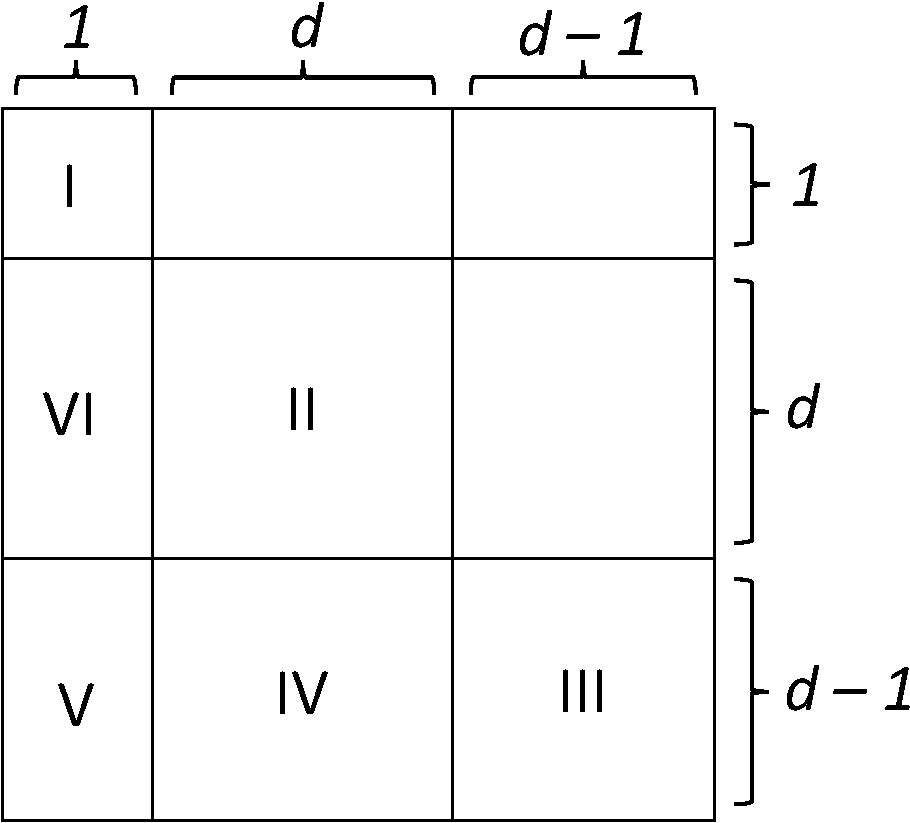
\includegraphics[width=0.6\linewidth]{fig2_crop}
	\caption{Block structure of matrix $J_z(\theta^{EM}; m, g)$.}
	\label{fig2crop}
\end{figure}
\noindent
\underline{Sub-matrix I}. Denote sub-matrix I by $J_z^{\pi}(\theta^{\textrm{EM}}; m, g).$ The formula for $J_z^{\pi}(\theta^{\textrm{EM}}; m, g)$ is 
\begin{multline}\label{sub_mat_1}
J^{\pi}_z(\theta^{\textrm{EM}}; m,g) = -\E \left[\nabla^2_\pi \mathcal{L}_z(\theta; m, g, p) \right] \\ + \left(\E\left[ \nabla_\pi \mathcal{L}_z(\theta; m, g, p) \right] \right)^2 - \E\left[ ( \nabla_\pi \mathcal{L}_z(\theta; m, g, p))^2 \right].
\end{multline}

We begin by calculating the first and second derivatives of the log-likelihood $\mathcal{L}_z$ with respect to $\pi$. We have that
\begin{multline*}
\frac{\partial }{\partial \pi } \mathcal{L}_z(\theta; m, g, p) = \frac{\partial }{\partial \pi } \left( \sum_{i=1}^n p_i \log(\pi) + \sum_{i=1}^n (1 - p_i) \log(1 - \pi) \right) \\ = \frac{ \sum_{i=1}^n p_i }{\pi} - \frac{ \sum_{i=1}^n (1 - p_i) }{ 1 - \pi } = \frac{\sum_{i=1}^n p_i}{\pi} - \frac{n - \sum_{i=1}^n p_i}{1 - \pi} \\ = \left( \frac{1}{\pi} + \frac{1}{1 - \pi} \right) \sum_{i=1}^n p_i - \frac{n}{1-\pi}.
\end{multline*}
Next, we compute the second derivative of $\mathcal{L}_z$ with respect to $\pi$:
\begin{multline*}
\frac{\partial^2}{\partial^2\pi} \mathcal{L}(\theta)  = \frac{\partial^2}{\partial^2\pi} \left( \frac{ \sum_{i=1}^n p_i }{ \pi } - \frac{ n - \sum_{i=1}^n p_i }{1 - \pi}  \right) = \frac{\left( \sum_{i=1}^n p_i \right) - n}{(1 - \pi)^2} - \frac{\sum_{i=1}^n p_i }{ \pi^2 }.
\end{multline*}
We compute the first expectation on the right-hand side of (\ref{sub_mat_1}).
\begin{multline*}
\E \left[ - \nabla^2_{\pi^{\textrm{EM}}} \mathcal{L}_z(\theta; m, g, x)\right] = - \E \left[ \frac{ ( \sum_{i=1}^n p_i) - n}{ (1 - \pi^{\textrm{EM}})^2} - \frac{ \sum_{i=1}^n p_i}{(\pi^{\textrm{EM}})^2} \right] \\ = - \E\left\{ \left[ \frac{1}{(1-\pi^{\textrm{EM}})^2} - \frac{1}{(\pi^{\textrm{EM}})^2} \right] \sum_{i=1}^n p_i - \frac{n}{ (1 - \pi^{\textrm{EM}})^2 } \right\} \\ = - \left\{ \left[ \frac{1}{(1-\pi^{\textrm{EM}})^2} - \frac{1}{(\pi^{\textrm{EM}})^2} \right] \sum_{i=1}^n T_i(1) - \frac{n}{ (1 - \pi^{\textrm{EM}})^2}  \right\} \\ = \left[ \frac{1}{(\pi^{\textrm{EM}})^2} - \frac{1}{ (1 - \pi^{\textrm{EM}})^2} \right] \sum_{i=1}^n T_i(1) + \frac{n}{(1-\pi^{\textrm{EM}})^2}.
\end{multline*}

Next, we compute the difference of the second two pieces of (\ref{sub_mat_1}). Define $$a := \frac{1}{(1-\pi^{\textrm{EM}})} + \frac{1}{\pi^{\textrm{EM}}}$$ and $$b := \frac{n}{(1-\pi^{\textrm{EM}})}.$$ We have that

\begin{multline*}
\E \left[ \nabla_\pi \mathcal{L}_z(\theta; m, g, x)^2 \right] = \E \left[ \left( a \sum_{i=1}^n p_i - b\right)^2 \right] =  \E \left[ a^2 \left( \sum_{i=1}^n p_i \right)^2 - 2ab \sum_{i=1}^n p_i + b^2 \right] \\ = a^2 \sum_{i=1}^n \sum_{j=1}^n \E[p_i p_j] -2ab \sum_{i=1}^n \E [p_i] + b^2.
\end{multline*}

Next,
\begin{multline*}
\left( \E \left[\nabla_\pi \mathcal{L}_z(\theta; m, g, x) \right] \right)^2 = \left( a \sum_{i=1}^n \E (p_i) - b \right)^2 = a^2 \sum_{i=1}^n \sum_{j=1}^n \E[p_i]  E[p_j] - 2ab \sum_{i=1}^n \E[p_i] + b^2.
\end{multline*}
Therefore,
\begin{multline*} ( \E [\nabla_\pi \mathcal{L}_z(\theta; m, g, x)])^2 - \E \left[\nabla_\pi \mathcal{L}_z(\theta; m, g, x)^2 \right] \\ = a^2 \sum_{i=1}^n \sum_{j=1}^n \E[p_i] \E[p_j] - a^2 \sum_{i=1}^n \sum_{j=1}^n \E[p_i p_j] = a^2 \left( \sum_{i=1}^n \E[p_i]^2 - \E[p_i^2]\right) \\ = a^2 \left( \sum_{i=1}^n [T_i(1)]^2 - T_i(1) \right) = \left( \frac{1}{(1 - \pi^{\textrm{EM}})} + \frac{1}{\pi^{\textrm{EM}}} \right)^2 \left( \sum_{i=1}^n [T_i(1)]^2 - T_i(1) \right).
\end{multline*}
Stringing these pieces together, we obtain
\begin{multline}\label{sub_mat_1_formula}
J_z^\pi(\theta^{\textrm{EM}}; m, g) = 
\left[ \frac{1}{(\pi^{\textrm{EM}})^2} - \frac{1}{ (1 - \pi^{\textrm{EM}} )^2} \right] \sum_{i=1}^n T_i(1) + \frac{n}{(1-\pi^{\textrm{EM}} )^2} \\ + \left( \frac{1}{(1 - \pi^{\textrm{EM}} )} + \frac{1}{\pi^{\textrm{EM}}} \right)^2 \left( \sum_{i=1}^n [T_i(1)]^2 - T_i(1) \right).
\end{multline}
\\
\underline{Sub-matrix II}. Denote sub-matrix II by $J_z^{\beta^m}(\theta^{EM}; m, g).$ The formula for $J_z^{\beta^m}(\theta^{EM}; m, g)$ is
\begin{multline}\label{sub_mat_2}
J^{\beta^m}_z(\theta^\textrm{EM}; m, g) = -\E \left[\nabla_{\beta^m}^2 \mathcal{L}_z(\theta; m, g, p) \right] \\ + \E\left[\nabla_{\beta^m} \mathcal{L}_z(\theta; m, g, p) \right] \E\left[ \nabla_{\beta^m} \mathcal{L}_z(\theta; m, g, p) \right]^T \\ - \E\left[ \nabla_{\beta^m} \mathcal{L}_z(\theta; m, g, p) \nabla_{\beta^m} \mathcal{L}_z(\theta; m, g, p)^T  \right].
\end{multline}
Now,
$$ -\nabla_{\beta^m}^2 \mathcal{L}_z(\theta; m, g, p) = \tilde{X}^T ( \Delta^m V^m \Delta^m - [\Delta']^m H^m ) \tilde{X}$$ and $$\nabla_{\beta^m}\mathcal{L}_z(\theta; m, g, p) = \tilde{X}^T \Delta^m s^m.$$

We compute the first term on the right-hand-side of (\ref{sub_mat_2}). The $(k,l)$th entry of this matrix is
\begin{multline*}
\left( \E\left[-\nabla_{\beta^m}^2 \mathcal{L}_z(\theta; m, g, p)\right]\right)[k,l] = \E \left\{\tilde{X}[,k]^T (\Delta^m V^m \Delta^m - [\Delta']^mH^m) \tilde{X}[,l] \right\} \\ = \sum_{i=1}^n \E \left\{ \tilde{x}_{i,k} (\Delta^m_{i} V^m_{i} \Delta^m_{i} - [\Delta']^m_{i} H^m_{i}) \tilde{x}_{i,l} \right\} \\ = \sum_{i=1}^n \tilde{x}_{i,k}(0) T_i(0) [{\Delta}^m_i(0)  {V}^m_i(0) {\Delta}^m_i(0) - [\Delta']^m_i(0) {H}^m_i(0)] \tilde{x}_{i,l}(0) \\ + \sum_{i=1}^n \tilde{x}_{i,k}(1) T_i(1) [ {\Delta}^m_i(1)  {V}^m_i(1) {\Delta}^m_i(1) - [{\Delta}']^m_i(1) {H}^m_i(1)] \tilde{x}_{i,l}(1) \\ = \sum_{s = 0}^1 \tilde{X}(s)[,k]^T {T}(s) \left[ {\Delta}^m(s) {V}^m(s) {\Delta}^m(s) - [{\Delta}']^m(s) {H}^m(s) \right] \tilde{X}(s)[,l].
\end{multline*}
We therefore have that
\begin{multline*} \E\left[-\nabla_{\beta^m}^2 \mathcal{L}_z(\theta; m, g, p)\right] \\ = \sum_{s=0}^1 \tilde{X}(s)^T T(s) \left[ {\Delta}^m(s) {V}^m(s) {\Delta}^m(s) - [{\Delta}']^m(s) {H}^m(s) \right] \tilde{X}(s).
\end{multline*}
Next, we compute the difference of the last two terms on the right-hand-side of (\ref{sub_mat_2}). The $(k,l)$th entry is
\begin{multline*}
[ \E \left[ \nabla_{\beta^m} \mathcal{L}_z(\theta; m, g, p) \right] \E \left[ \nabla_{\beta^m} \mathcal{L}_z(\theta; m, g, p) \right]^T \\ - \E \left[ \nabla_{\beta^m} \mathcal{L}_z(\theta; m, g, p) \nabla_{\beta^m} \mathcal{L}_z(\theta; m, g, p)^T \right] ][k,l] \\ 
= \left[ \E \left[\tilde{X}^T \Delta^m s^m \right] \E \left[\tilde{X}^T \Delta^m s^m \right]^T\right][k,l] - \E \left[\tilde{X}^T \Delta^m s^m (s^m)^T \Delta^m \tilde{X} \right][k,l] \\
= \E\left[ \tilde{X}[,k]^T \Delta^m s^m \right] \E \left[ \tilde{X}[,l]^T \Delta^m s^m \right] - \E \left[ \tilde{X}[,k]^T \Delta^m s^m (s^m)^T \Delta^m \tilde{X}[,l ] \right] \\ 
=\E\left(\sum_{i=1}^n \tilde{x}_{ik} \Delta^m_i s^m_{i} \right) \E \left( \sum_{j=1}^n \tilde{x}_{jl} \Delta^m_j s^m_j \right) - \E \left( \sum_{i=1}^n \sum_{j=1}^n \tilde{x}_{ik} \Delta^m_i s^m_i s^m_j \Delta^m_j \tilde{x}_{jl} \right) \\ 
= \sum_{i=1}^n \sum_{j=1}^n \E[ \tilde{x}_{ik} \Delta^m_is^m_i] \E [\tilde{x}_{jl} \Delta^m_j s^m_j]  -  \sum_{i=1}^n \sum_{j=1}^n \E [ \tilde{x}_{ik} \Delta^m_i s^m_i s^m_j \Delta^m_j \tilde{x}_{jl}] \\
= \sum_{i=1}^n \sum_{j=1}^n \E[ \tilde{x}_{ik} \Delta^m_i s^m_i] \E \left[\tilde{x}_{jl} \Delta^m_j s^m_j \right]  - \sum_{i \neq j} \E [ \tilde{x}_{ik} \Delta^m_i s^m_i] \E[s^m_j \Delta^m_j \tilde{x}_{jl}] - \sum_{i=1}^n \E[\tilde{x}_{ik} \Delta^m_i s^m_i s^m_i \Delta^m_i \tilde{x}_{il}] \\ 
= \sum_{i=1}^n \E[\tilde{x}_{ik} \Delta^m_i s^m_i ] \E [ \tilde{x}_{il} \Delta^m_i s^m_i] - \sum_{i=1}^n \E[\tilde{x}_{ik} (\Delta_i^m)^2 (H_i^m)^2 \tilde{x}_{il}] \\ = \sum_{i=1}^n \left[\tilde{x}_{ik}(0) {\Delta}^m_i(0) T_i(0) {H}^m_i(0) + \tilde{x}_{ik}(1) {\Delta}^m_i(1) T_i(1) {H}^m_i(1) \right] \\ \cdot \left[ \tilde{x}_{il}(0) {\Delta}^m_i(0) T_i(0) {H}^m_i(0) + \tilde{x}_{il}(1) {\Delta}^m_i(1) T_i(1) {H}^m_i(1) \right] \\ - \sum_{i=1}^n \left[ \tilde{x}_{ik}(0) T_i(0) (\Delta_i^m(0))^2 ({H}_i^m(0))^2 \tilde{x}_{il}(0)  + \tilde{x}_{ik}(1) T_i(1) ({\Delta}^m_i(1))^2 ({H}_i^m(1))^m \tilde{x}_{il}(1) \right] \\ = \sum_{s=0}^1 \sum_{t=0}^1 \left[ \sum_{i=1}^n \tilde{x}_{ik}(s) T_i(s) {\Delta}^m_i(s) {H}^m_i(t) T_i(t){\Delta}^m_i(t) {H}^m_i(t) \tilde{x}_{il}(t) \right] \\ - \sum_{s=0}^1 \left[\sum_{i=1}^n \tilde{x}_{ik}(s) T_i(s) ({\Delta}^m_i(s))^2 ({H}_i^m(s))^2 \tilde{x}_{il}(s) \right] \\ = \sum_{s=0}^1 \sum_{t=0}^1 \tilde{X}(s)[,k]^T {T}(s) {\Delta}^m(s) {H}^m(s) {T}(t) {\Delta}^m(t) {H}^m(t) \tilde{X}(k)[,l] \\ - \sum_{s=0}^1{X}(s)[,k]^T {T}(s) ({\Delta}^m(s))^2 ({H}^m(s))^2 \tilde{X}(s)[,l].
\end{multline*}
The sum of the last two terms on the right-hand side of (\ref{sub_mat_2}) is therefore
\begin{multline*} \sum_{s=0}^1 \sum_{t=0}^1 \tilde{X}(s)^T {T}(s) {\Delta}^m(s) {H}^m(s) {T}(t) {\Delta}^m(t) {H}^m(t) \tilde{X}(t) \\ - \sum_{s=0}^1 \tilde{X}(s)^T {T}(s) ({\Delta}^m(s))^2 ({H}^m(s))^2 \tilde{X}(s). \end{multline*}
Stringing everything together, we find
\begin{multline}\label{sub_mat_2_formula}
J_z^{\beta^m}(\theta^{EM}; m, g) = \sum_{s=0}^1 \tilde{X}(s)^T T(s) \left[ {\Delta}^m(s) {V}^m(s) {\Delta}^m(s) - [{\Delta}']^m(s) {H}^m(s) \right] \tilde{X}(s) + \\ \sum_{s=0}^1 \sum_{t=0}^1 \tilde{X}(s)^T {T}(s) {\Delta}^m(s) {H}^m(s) {T}(t) {\Delta}^m(t) {H}^m(t) \tilde{X}(t) \\ - \sum_{s=0}^1 \tilde{X}(s)^T {T}(s) ({\Delta}^m(s))^2 ({H}^m(s))^2 \tilde{X}(s).
\end{multline}
\\
\noindent \underline{Sub-matrix III}. Denote sub-matrix III by $J_z^{\beta^g}(\theta^{EM}; m, g).$ The formula for $J_z^{\beta^g}(\theta^{EM}; m, g)$ is
\begin{multline}\label{sub_mat_3}
J^{\beta^g}_z(\theta^\textrm{EM}; m, g) = -\E \left[\nabla_{\beta^{(g,z)}}^2 \mathcal{L}_z(\theta; m, g, p) \right] \\ + \E\left[ \nabla_{\beta^{(g,z)}} \mathcal{L}_z(\theta; m, g, p) \right] \E\left[\nabla_{\beta^{(g,z)}} \mathcal{L}_z(\theta; m, g, p) \right]^T \\ - \E\left[ \nabla_{\beta^{(g,z)}} \mathcal{L}_z(\theta; m, g, p) \nabla_{\beta^{(g,z)}} \mathcal{L}_z(\theta; m, g, p)^T \right].
\end{multline}
We have that
$$ -\nabla_{\beta^{(g,z)}}^2 \mathcal{L}_z(\theta; m, g, p) =  X^T P ( \Delta^{(g,z)}V^{(g,z)}\Delta^{(g,z)} - (\Delta')^{(g,z)} H^{(g,z)}) X$$ and
$$ \nabla_{\beta^{(g,z)}} \mathcal{L}_z(\theta; m, g, p) = X^T P \Delta^{(g,z)} s^{(g,z)}.$$

We compute the first entry on the right-hand-side of (\ref{sub_mat_3}). The only random matrix among $X, P, \Delta^{(g,z)}, V^{(g,z)}, (\Delta')^{(g,z)},$ and $H^{(g,z)}$ is $P$. Therefore, by linearity of expectation,
\begin{multline*}
\E \left[ X^T P (\Delta^{(g,z)}V^{(g,z)}\Delta^{(g,z)} - (\Delta')^{(g,z)} H^{(g,z)} \right] \\ = X^T T(1) ( \Delta^{(g,z)}V^{(g,z)}\Delta^{(g,z)} - (\Delta')^{(g,z)} H^{(g,z)}) X.
\end{multline*}
Next, we compute the difference of the last two terms on the right-hand-side of (\ref{sub_mat_3}). The $(k,l)$th entry of this matrix is
\begin{multline*}
[ \E \left[ \nabla_{\beta^g} \mathcal{L}_z(\theta; m, g, p) \right] \E \left[ \nabla_{\beta^g} \mathcal{L}_z(\theta; m, g, p) \right]^T - \E \left[ \nabla_{\beta^g} \mathcal{L}_z(\theta; m, g, p) \nabla_{\beta^g} \mathcal{L}_z(\theta; m, g, p)^T \right] ][k,l] \\ 
= \left[ \E \left[ {X}^T P \Delta^{(g,z)} s^{(g,z)} \right]\E \left[ {X}^T P \Delta^{(g,z)} s^{(g,z)} \right]^T\right][k,l] - \E \left[ {X}^T P \Delta s^{(g,z)} (s^{(g,z)})^T \Delta^{(g,z)} P {X}^T \right][k,l] \\ 
= \E\left[{X}[,k]^T P \Delta^{(g,z)} s^{(g,z)} \right] \E \left[ {X}[,l]^T P \Delta^{(g,z)} s^{(g,z)} \right] - \E \left[ {X}[,k]^T P \Delta^{(g,z)} s^{(g,z)} (s^{(g,z)})^T \Delta^{(g,z)} P {X}[,l ] \right] \\
=\E\left(\sum_{i=1}^n {x}_{ik} P_i \Delta^{(g,z)}_i s^{(g,z)}_{i} \right) \E \left( \sum_{j=1}^n {x}_{jl} P_j \Delta^{(g,z)}_j s^{(g,z)}_j \right) \\ - \E \left( \sum_{i=1}^n \sum_{j=1}^n {x}_{ik} P_i \Delta^{(g,z)}_i s^{(g,z)}_i s^{(g,z)}_j \Delta^{(g,z)}_j P_j{x}_{jl} \right) \\ 
= \sum_{i=1}^n \sum_{j=1}^n \E[ {x}_{ik} P_i \Delta^{(g,z)}_is^{(g,z)}_i] \E [ {x}_{jl} P_j \Delta^{(g,z)}_j s^{(g,z)}_j]  -  \sum_{i=1}^n \sum_{j=1}^n \E [ {x}_{ik} P_i \Delta^{(g,z)}_i s^{(g,z)}_i s^{(g,z)}_j \Delta^{(g,z)}_jP_j {x}_{jl}  ]  \\
= \sum_{i=1}^n \sum_{j=1}^n \E[ {x}_{ik} P_i \Delta^{(g,z)}_i s^{(g,z)}_i ] \E \left[{x}_{jl} P_j \Delta^{(g,z)}_j s^{(g,z)}_j \right]  - \sum_{i \neq j} \E [{x}_{ik} P_i \Delta^{(g,z)}_i s^{(g,z)}_i] \E[s^{(g,z)}_j P_j \Delta^{(g,z)}_j {x}_{jl}] \\ - \sum_{i=1}^n \E[ {x}_{ik}P_i \Delta^{(g,z)}_i s^{(g,z)}_i s^{(g,z)}_i \Delta^{(g,z)}_i P_i{x}_{il}] \\ 
= \sum_{i=1}^n \E[ {x}_{ik} P_i \Delta^{(g,z)}_i H^{(g,z)}_i] \E[{x}_{il}P_i\Delta^{(g,z)}_i H^{(g,z)}_i] - \sum_{i=1}^n \E[{x}_{ik}P_i^2(\Delta^{(g,z)}_i)^2 (H^{(g,z)}_i)^2 {x}_{il}] \\ = \sum_{i=1}^n {x}_{ik} T_i(1)^2(\Delta^{(g,z)}_i)^2 (H_i^{(g,z)})^2{x}_{il} - \sum_{i=1}^n {x}_{ik} T_i(1) (\Delta_i^{(g,z)})^2 (H_i^{(g,z)})^2 {x}_{il} \\ = {X}[,k]^T T(1)^2 (\Delta^{(g,z)})^2 (H^{(g,z)})^2 {X}[,l] - {X}[,k]^T T(1) (\Delta^{(g,z)})^2 (H^{(g,z)})^2 {X}[,l]
\end{multline*}
Therefore, the difference of the last two terms of the right-hand-side of (\ref{sub_mat_3}) is
\begin{multline*} X^T T(1)^2 (\Delta^{(g,z)})^2(H^{(g,z)})^2{X} - {X}^T T(1) (\Delta^{(g,z)})^2 (H^{(g,z)})^2 {X} \\ = - X^T T(1) \left(\Delta^{(g,z)}\right)^2 \left( H^{(g,z)} \right)^2 \left( I - T(1)  \right) X. \end{multline*}
Stringing these pieces together, we have that
\begin{multline}\label{sub_mat_3_formula}
J^{\beta^g}_z\left( \theta^{\textrm{EM}}; m, g \right) =  X^T T(1) ( \Delta^{(g,z)}V^{(g,z)}\Delta^{(g,z)} - (\Delta')^{(g,z)} H^{(g,z)}) X \\ - X^T T(1) \left(\Delta^{(g,z)}\right)^2 \left( H^{(g,z)} \right)^2 \left( I - T(1) \right) X.
\end{multline}
\underline{Sub-matrix IV}.  Denote sub-matrix IV by
 $J^{(\beta^{g}, \beta^m)}_z(\theta^{\textrm{EM}}; m, g).$ The formula for $J^{(\beta^{g}, \beta^m)}_z(\theta^{\textrm{EM}}; m, g)$ is
\begin{multline}\label{sub_mat_4}
J^{(\beta^g, \beta^m)}_z(\theta^{\textrm{EM}}; m, g)= - \E \left[\nabla_{\beta^{(g,z)}} \nabla_{\beta^m} \mathcal{L}_z (\theta; m, g, p) \right] \\ + \E\left[ \nabla_{\beta^{(g,z)} }\mathcal{L}_z(\theta ; m,g,p) \right]\E\left[\nabla_{\beta^m}\mathcal{L}_z(\theta; m,g,p)\right]^T \\ - \E \left[\nabla_{\beta^{(g,z)}}\mathcal{L}_z (\theta; m,g,p) \nabla_{\beta^m}\mathcal{L}_z(\theta; m,g,p)]^T \right].
\end{multline} Recall that $\nabla_{\beta^{(g,z)}} \mathcal{L}_z(\theta; m, g, p) = X P \Delta^{(g,z)} s^{(g,z)}$ and $\nabla_{\beta^m} \mathcal{L}_z(\theta; m, g, p) = \tilde{X} \Delta^m s^m.$ The first term on the right-hand side of (\ref{sub_mat_4}) is $0$. We compute the difference of the last two terms. Entry $(k,l)$ of this matrix is
\begin{multline*}
[\E[\nabla_{\beta^{(g,z)}}\mathcal{L}_z(\theta; m, g, p) ] \E [\nabla_{\beta^m} \mathcal{L}_z(\theta; m, g, p) ]^T \\ - \E [\nabla_{\beta^{(g,z)}} \mathcal{L}_z(\theta; m, g, p) \nabla_{\beta^m}\mathcal{L}_z(\theta; m, g, p)^T ] ][k,l] \\ 
= \left[ \E \left[ {X}^T P \Delta^{(g,z)} s^{(g,z)} \right] \E\left[\tilde{X}^T \Delta^m s^m\right]^T\right][k,l] - \E \left[{X}^T P \Delta^{(g,z)} s^{(g,z)} (s^m)^T \Delta^m \tilde{X} \right][k,l] \\ = \left[\E\left[{X}[,k]^T P \Delta^{(g,z)} s^{(g,z)}\right]\E\left[\tilde{X}[,l]^T \Delta^m s^m\right]^T\right] - \E \left[{X}[,k]^T P \Delta^{(g,z)} s^{(g,z)} (s^m)^T \Delta^m \tilde{X}[,l] \right] \\ = \E\left(\sum_{i=1}^n x_{ik} P_i \Delta^{(g,z)}_i s^{(g,z)}_i\right) \E \left(\sum_{j=1}^n \tilde{x}_{jl} \Delta^m_j s^m_j \right) - \E \left(\sum_{i=1}^n \sum_{j=1}^n x_{ik} P_i \Delta^{(g,z)}_i s^{(g,z)}_i \Delta^m_j s^m_j \tilde{x}_{jl}  \right) \\ 
= \sum_{i=1}^n \sum_{j=1}^n \E [x_{ik} P_i \Delta^{(g,z)}_i s^{(g,z)}_i] \E[\Delta^m_js^m_j \tilde{x}_{jl}] - \sum_{i=1}^n \sum_{j=1}^n \E[x_{ik} P_i \Delta^{(g,z)}_i s^{(g,z)}_i \Delta^m_j s^m_j \tilde{x}_{jl}] \\
= \sum_{i=1}^n \sum_{j=1}^n \E [x_{ik} P_i \Delta^{(g,z)}_i s^{(g,z)}_i ] \E[\Delta^m_js^m_j \tilde{x}_{jl}] - \sum_{i \neq j} \E [x_{ik} P_i \Delta^{(g,z)}_i s^{(g,z)}_i] \E[\Delta^m_js^m_j \tilde{x}_{jl}] \\ - \sum_{i=1}^n \E[x_{ik} P_i \Delta^{(g,z)}_i s^{(g,z)}_i \Delta^m_j s^m_j \tilde{x}_{jl}] \\
= \sum_{i=1}^n \E[x_{ik} P_i \Delta_i^{(g,z)} H^{(g,z)}_i] \E[\tilde{x}_{il} \Delta^m_i H^m_i] - \sum_{i=1}^n \E[x_{ik} P_i \Delta_i^{(g,z)} H_i^{(g,z)} \Delta_i^m H_i^m \tilde{x}_{il}] \\ 
= \sum_{i=1}^n \left[x_{ik} T_i(1) \Delta^{(g,z)}_i H^{(g,z)}_i \right] \cdot \left[{\Delta}^m_i(0) T_i(0) {H}^m_i(0) \tilde{x}_{il}(0) + {\Delta}^m_i(1) T_i(1) {H}^m_i(1) \tilde{x}_{il}(1)\right]
\\ - \sum_{i=1}^n \left[x_{ik} T_i(1) \Delta^{(g,z)}_i H^{(g,z)}_i \Delta^m_i(1) H^m_i(1) \tilde{x}_{il}(1)\right] 
\\ = \sum_{s=0}^1 \sum_{i=1}^n x_{ik} T_i(1) H_i^{(g,z)} \Delta_i^{(g,z)} T_i(s) \Delta_i^m(s) H^m(s) \tilde{x}_{il}(s) \\ - \sum_{i=1}^n \left[x_{il}T_i(1) \Delta^{(g,z)}_i H^{(g,z)}_i \Delta^m_i(1) H^m_i(1) \tilde{x}_{ik}(1)\right] \\ = \sum_{s=0}^1 X[,k]^T T(1) H^{(g,z)} \Delta^{(g,z)} T(s)\Delta^m(s)H^m(s) \tilde{X}(s)[,l] \\ - X[,k]^T \Delta^{(g,z)} H^{(g,z)} T(1)\Delta^m(1) H^m(1) \tilde{X}[,l].
\end{multline*}
We finally conclude that 
\begin{multline}\label{sub_mat_4_formula} J_z^{(\beta^m, \beta^g)}(\theta; m, g) = \left(\sum_{s=0}^1 X^T  T(1) H^{(g,z)} \Delta^{(g,z)} T(s) \Delta^m(s) H^m(s) \tilde{X}(s) \right) \\ - X^T \Delta^{(g,z)} H^{(g,z)} T(1) \Delta^m(1)H^m(1) \tilde{X}(1).
\end{multline}
\noindent
\underline{Sub-matrix V}. Denote sub-matrix V by $J_z^{(\beta^g,\pi)}(\theta; m, g).$ The formula for $J_z^{(\beta^g,\pi)}(\theta; m, g)$ is
\begin{multline}\label{sub_mat_5}
J_{(\beta^g,\pi)}(\theta; m,g) = \E \left[-\nabla_{\beta^{(g,z)}} \nabla_{\pi} \mathcal{L}_z(\theta; m, g, p) \right] \\ + \E\left[ \nabla_{\beta^{(g,z)}}\mathcal{L}_z(\theta; m, g ,p)\right] \E \left[ \nabla_{\pi}\mathcal{L}_z(\theta; m,g,p) \right] \\ - \E \left[ \nabla_{\beta^{(g,z)}}\mathcal{L}_z(\theta; m,g,p) \nabla_{\pi}\mathcal{L}_z(\theta; m,g,p) \right].
\end{multline} Recall that $\nabla_{\beta^{(g,z)}} \mathcal{L}_z(\theta; m, g, p) = X^T P \Delta^{(g,z)}s^{(g,z)}$ and $$ \nabla_\pi \mathcal{L}_z(\theta; m, g, p) = \left( \frac{1}{\pi} + \frac{1}{1 - \pi} \right) \left(\sum_{i=1}^n p_i\right)  - \frac{n}{1 - \pi}.$$  Set $$a = \frac{1}{\pi^\textrm{EM}} + \frac{1}{1 - \pi^\textrm{EM}}, \textrm{    } b = \frac{n}{1 - \pi^\textrm{EM}}.$$ The first term on the right-hand-side of (\ref{sub_mat_5}) is $0$. We compute the difference of the last two terms. The $k$th entry of this vector is
\begin{multline*}
\E \left[ \nabla_\pi \mathcal{L}_z(\theta; m, g, p) \right] \E\left[\nabla_{\beta^{(g, z)}} \mathcal{L}_z(\theta; m, g, x)[k] \right] - \E \left[\nabla_{\pi}\mathcal{L}(\theta; m,g,p) \nabla_{\beta^{(g,z)}} \mathcal{L} (\theta; m,g,p)[k] \right] \\= \left(\E \left[ a \sum_{i=1}^n p_i - b \right] \right)\left( \E \left[{X}[,k]^T P \Delta^{(g,z)} s^{(g,z)} \right]\right) - \E \left[ \left( a \sum_{i=1}^n p_i - b \right) {X}[,k]^T P \Delta^{(g,z)} s^{(g,z)}\right] \\ = \left( a \sum_{i=1}^n \E[p_i] - b \right) \left( \sum_{j=1}^n \E [x_{jk} p_j \Delta^{(g,z)}_j s^{(g,z)}_j] \right) \\ - \E \left[ \left( a \sum_{i=1}^n p_i - b \right) \left( \sum_{j=1}^n \tilde{x}_{jk} p_j \Delta^{(g,z)}_j s^{(g,z)}_j \right) \right] \\= a \sum_{i=1}^n \sum_{j=1}^n \E [p_i] \E[x_{jk} p_j \Delta^{(g,z)}_j s^{(g,z)}_j] - b \sum_{j=1}^n \E[x_{jk} p_j \Delta^{(g,z)}_j s^{(g,z)}_j] \\ - \left[a \sum_{i=1}^n \sum_{j=1}^n \E [ p_i x_{jk} p_j \Delta^{(g,z)}_j s^{(g,z)}_j] - b \sum_{j=1}^n \E[x_{jk} p_j \Delta^{(g,z)}_j s^{(g,z)}_j] \right] \\ = a \sum_{i=1}^n \sum_{j=1}^n \E[p_i] \E[{x}_{jk} p_j \Delta^{(g,z)}_j s^{(g,z)}_j] - a \sum_{i \neq j} \E[p_i] \E[x_{jk} p_j \Delta^{(g,z)}_j s^{(g,z)}_j] - a \sum_{i=1}^n \E[ x_{ik} p_i^2 \Delta^{(g,z)}_i s^{(g,z)}_i] \\ = a \sum_{i=1}^n \E[p_i] \E[x_{ik} p_i \Delta^{(g,z)}_i s^{(g,z)}_i] - a \sum_{i=1}^n \E[x_{ik} p_i^2 \Delta^{(g,z)}_i s^{(g,z)}_i] \\ = a \sum_{i=1}^n T_i(1) x_{ik} T_i(1) \Delta^{(g,z)}_i s^{(g,z)}_i - a \sum_{i=1}^n x_{ik} T_i(1) \Delta^{(g,z)}_i s^{(g,z)}_i \\ = a \sum_{i=1}^n \left( {x}_{ik} T_i(1)^2 \Delta^{(g,z)}_i s^{(g,z)}_i - x_{ik} T_i(1) \Delta^{(g,z)}_i s^{(g,z)}_i \right) = a \sum_{i=1}^n {x}_{ik}T_i(1)\Delta^{(g,z)}_i s^{(g,z)}_i \left( T_i(1) - 1\right) \\ = -a\sum_{i=1}^n x_{ik} T_i(0) T_i(1)\Delta^{(g,z)}_i H^{(g,z)}_i = -a X[,k]^T w^{(g,z)}.
\end{multline*}
We conclude that
\begin{equation}\label{sub_mat_5_formula} J^{(\beta^g, \pi)}_z(\theta; m, g) = -\left( \frac{1}{\pi^\textrm{EM}} + \frac{1}{1-\pi^\textrm{EM}} \right)X^T w^{(g,z)}. \end{equation}
\\
\noindent
\underline{Sub-matrix VI}. Denote sub-matrix VI by $J_z^{(\beta^m,\pi)}(\theta; m, g).$ The formula for $J_z^{(\beta^m,\pi)}(\theta; m, g)$ is
\begin{multline}\label{sub_mat_6}
J_z^{(\beta^m,\pi)}(\theta; m, g) = \E \left[ - \nabla_{\beta^m} \nabla_{ \pi } \mathcal{L}_z(\theta; m, g, p) \right] + \E\left[ \nabla_{\beta^m}\mathcal{L}_z(\theta ; m,g,p) \right] \E \left[ \nabla_{\pi}\mathcal{L}_z(\theta ; m,g,p) \right]^T \\ - \E \left[ \nabla_{\beta^m}\mathcal{L}_z(\theta; m,g,p) \nabla_{\pi}\mathcal{L}_z(\theta; m,g,p)^T \right].
\end{multline} Recall that $ \nabla_{\beta^m} \mathcal{L}_z(\theta; m, g, p) = \tilde{X}^T \Delta^m s^m$. Again, set $a = 1/(\pi^\textrm{EM}) + 1/(1 - \pi^\textrm{EM})$ and $b = n/(1 - \pi^\textrm{EM}).$ The first term on the right-hand-side of (\ref{sub_mat_6}) is $0$. We compute the difference of the last two terms. The $k$th entry of this vector is
\begin{multline*}
\E \left[ \nabla_\pi \mathcal{L}_z(\theta; m, g, p) \right] \E\left[ \nabla_{\beta} \mathcal{L}_z(\theta; m, g, p)[k] \right] - \E \left[\nabla_{\pi}\mathcal{L}_z(\theta; m,g,p) \nabla_{\beta}\mathcal{L}_z(\theta; m,g,p)[k] \right] \\= \left(\E \left[ a \sum_{i=1}^n p_i - b \right] \right) \left(\E\left[ \tilde{X}[,k]^T \Delta^m s^m \right] \right) - \E \left[ \left( a \sum_{i=1}^n p_i - b \right) \tilde{X}[,k]^T \Delta^m s^m \right] \\ = \left( a \sum_{i=1}^n \E[p_i] - b \right) \left( \sum_{j=1}^n \E [ \tilde{x}_{jk}\Delta^m_js^m_j] \right) - \E \left[ \left( a \sum_{i=1}^n p_i - b \right) \left( \sum_{j=1}^n \tilde{x}_{jk} \Delta^m_j s^m_j \right) \right] \\ a \sum_{i=1}^n \sum_{j=1}^n \E [p_i] \E[ \tilde{x}_{jk} \Delta^m_j s^m_j] - b \sum_{j=1}^n \E[\tilde{x}_{jk} \Delta^m_j s^m_j] - \left[ a \sum_{i=1}^n \sum_{j=1}^n \E [ p_i \tilde{x}_{jk} \Delta^m_j s^m_j] - b \sum_{j=1}^n \E[\tilde{x}_{jk} \Delta^m_j s^m_j] \right] \\ =  a \sum_{i=1}^n \sum_{j=1}^n \E[p_i] \E[\tilde{x}_{jk} \Delta^m_j s^m_j] - a\sum_{i \neq j} \E[p_i] \E[\tilde{x}_{jk} \Delta^m_j s^m_j] - a\sum_{i=1}^n \E[ p_i \tilde{x}_{ik} \Delta^m_i s^m_i ] \\ = a \sum_{i=1}^n \E[p_i] \E[ \tilde{x}_{ik} \Delta^m_i s^m_i] - a \sum_{i=1}^n \E[p_i \tilde{x}_{ik} \Delta^m_i s^m_i] \\ = a \sum_{i=1}^n T_i(1) [T_i(0) \Delta^m_i(0) s^m_i(0) \tilde{x}_{ik}(0) + T_i(1) \Delta^m_i(1) s^m_i(1) \tilde{x}_{ik}(1)] \\ - a \sum_{i=1}^n T_i(1)\Delta^m_i(1)s^m_i(1)\tilde{x}_{ik}(1) \\ = a \sum_{i=1}^n T_i(0)T_i(1) \Delta_i^m(0)H^m_i(0)\tilde{x}_{ik}(0) \\ + a \sum_{i=1}^n \left( [T_i(1)]^2 \Delta^m_i(1)H^m_i(1) - T_i(1)\Delta^m_i(1)H^m_i(1) \right) \tilde{x}_{ik}(1)  \\ =a \left[ \sum_{i=1}^n T_i(0) T_i(1) \Delta^m_i(0) H^m_i(0) \tilde{x}_{ik}(0) + \sum_{i=1}^n T_i(1)\Delta^m_i(1)H^m_i(1)[T_i(1) - 1] \tilde{x}_{ik}(1) \right] \\ = a \left[ \sum_{i=1}^n T_i(0) T_i(1) \Delta^m_i(0) H^m_i(0) \tilde{x}_{ik}(0) - \sum_{i=1}^n T_i(0) T_i(1) \Delta^m_i(1) H^m_i(1) \tilde{x}_{ik}(1) \right] \\ = a\left(\tilde{X}(0)[,k]^T w^m(0) - \tilde{X}(1)[,k]^T w^m(1)  \right).
\end{multline*}
We conclude that
\begin{equation}\label{sub_mat_6_formula} J^{(\beta^m, \pi)}_z(\theta; m, g, p) = \left( \frac{1}{\pi^\textrm{EM}} + \frac{1}{1 - \pi^\textrm{EM}} \right) \left( \tilde{X}(0)^T w^m(0) - \tilde{X}(1)^T w^m(1)\right). \end{equation}
 \\ \noindent
\underline{Summary}: We derived formulas for sub-matrices I-VI (\ref{sub_mat_1}, \ref{sub_mat_2}, \ref{sub_mat_3}, \ref{sub_mat_4}, \ref{sub_mat_5}, \ref{sub_mat_6}). We list those formulas here:

\begin{itemize}
\item[I.] \begin{multline*}
J_z^\pi(\theta^{\textrm{EM}}; m, g) = 
\left[ \frac{1}{(\pi^{\textrm{EM}})^2} - \frac{1}{ (1 - \pi^{\textrm{EM}} )^2} \right] \sum_{i=1}^n T_i(1) + \frac{n}{(1-\pi^{\textrm{EM}} )^2} \\ + \left( \frac{1}{(1 - \pi^{\textrm{EM}} )} + \frac{1}{\pi^{\textrm{EM}}} \right)^2 \left( \sum_{i=1}^n [T_i(1)]^2 - T_i(1) \right).
\end{multline*}
\item[II.] \begin{multline*}
J_z^{\beta^m}(\theta^{EM}; m, g) = \sum_{s=0}^1 \tilde{X}(s)^T T(s) \left[ {\Delta}^m(s) {V}^m(s) {\Delta}^m(s) - [{\Delta}']^m(s) {H}^m(s) \right] \tilde{X}(s)  \\ + \sum_{s=0}^1 \sum_{t=0}^1 \tilde{X}(s)^T {T}(s) {\Delta}^m(s) {H}^m(s) {T}(t) {\Delta}^m(t) {H}^m(t) \tilde{X}(t) \\ - \sum_{s=0}^1 \tilde{X}(s)^T {T}(s) ({\Delta}^m(s))^2 ({H}^m(s))^2 \tilde{X}(s).
\end{multline*}
\item[III.] \begin{multline*}
J^{\beta^g}_z\left( \theta^{\textrm{EM}}; m, g \right) =  X^T T(1) ( \Delta^{(g,z)}V^{(g,z)}\Delta^{(g,z)} - (\Delta')^{(g,z)} H^{(g,z)}) X \\ - X^T T(1) \left(\Delta^{(g,z)}\right)^2 \left( H^{(g,z)} \right)^2 \left( I - T(1) \right) X.
\end{multline*}
\item[IV.] \begin{multline*} J_z^{(\beta^m, \beta^g)}(\theta; m, g) = \left(\sum_{s=0}^1 X^T  T(1) H^{(g,z)} \Delta^{(g,z)} T(s) \Delta^m(s) H^m(s) \tilde{X}(s) \right) \\ - X^T \Delta^{(g,z)} H^{(g,z)} T(1) \Delta^m(1)H^m(1) \tilde{X}(1).
\end{multline*}
\item[V.] \begin{equation*} J^{(\beta^g, \pi)}_z(\theta; m, g) = -\left( \frac{1}{\pi^\textrm{EM}} + \frac{1}{1-\pi^\textrm{EM}} \right)X^T w^{(g,z)}. \end{equation*}
\item[VI.] \begin{equation*} J^{(\beta^m, \pi)}_z(\theta; m, g, p) = \left( \frac{1}{\pi^\textrm{EM}} + \frac{1}{1 - \pi^\textrm{EM}} \right) \left( \tilde{X}(0)^T w^m(0) - \tilde{X}(1)^T w^m(1)\right). \end{equation*}
\end{itemize}

\subsection{Observed information matrix for background-read model}
 
Next, we calculate the information matrix for the background-read model. Let $J_b(\theta^\textrm{EM}; m, g)$ denote the observed information matrix for the background-read model based on $(m,g)$ evaluated at $\theta^\textrm{EM}.$ We have by (\ref{Louis_formula}) that
\begin{multline*}
J_b(\theta^\textrm{EM}; m, g) = -\E \left[\nabla^2 \mathcal{L}_b(\theta; m, g, p) | G = g, M = m, \theta^\textrm{EM} \right] \\ + \E\left[ \nabla \mathcal{L}_b(\theta; m, g, p) | G = g, M = m, \theta^\textrm{EM} \right] \E\left[ \nabla \mathcal{L}_b(\theta; m, g, p) | G = g, M = m, \theta^\textrm{EM} \right]^T \\ - \E\left[ \nabla\mathcal{L}_b(\theta; m, g, p) \nabla \mathcal{L}_z(\theta; m, g, p)^T | G = g, M = m, \theta^\textrm{EM} \right].
\end{multline*}
\begin{figure}
	\centering
	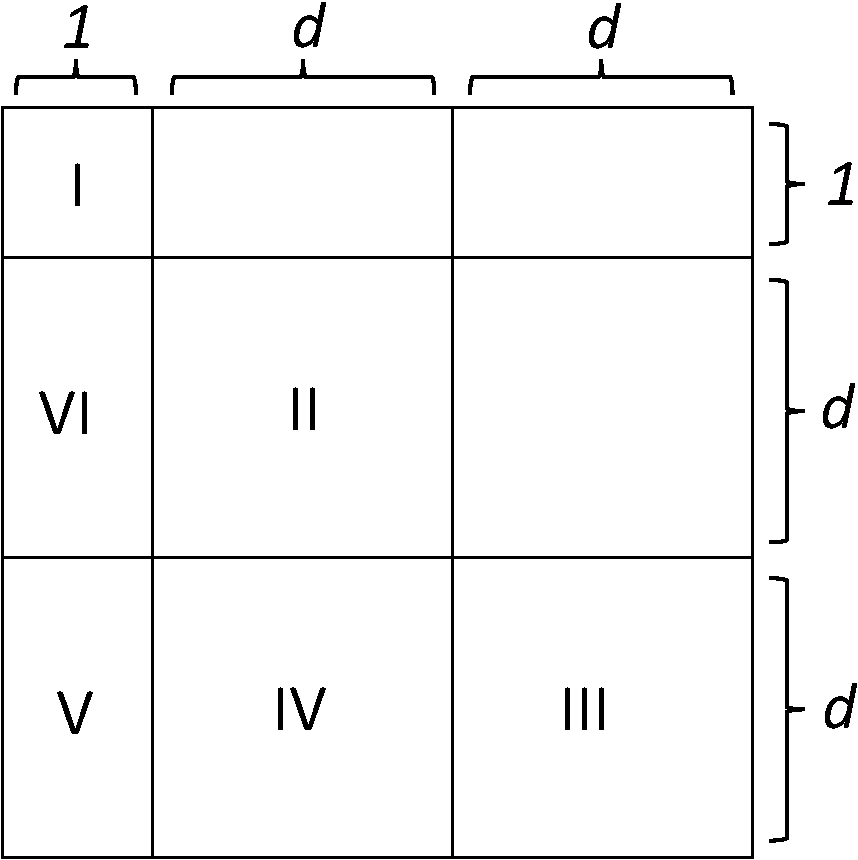
\includegraphics[width=0.6\linewidth]{fig3_crop}
	\caption{Block structure of matrix $J_b(\theta^{EM}; m, g)$.}
	\label{fig3crop}
\end{figure}
The matrix $J_b(\theta^\textrm{EM}; m, g)$ has dimension $(2d + 1) \times (2d + 1)$. We can partition $J(\theta^\textrm{EM}; m, g)$ into nine-submatrices (Figure \ref{fig3crop}). We compute these sub-matrices separately, saving effort by invoking proofs from the previous section (\ref{zero_inf_info_mat_sec}) when possible. Again, in what follows, all expectations are understood to be conditional on $M = m, G = g$, setting $\theta = \theta^{\textrm{EM}}.$ 
 \noindent \\ \\
 \underline{Sub-matrix I}. Denote sub-matrix I by $J_b^{\pi}(\theta^{\textrm{EM}}; m, g).$ The expression for sub-matrix I in the background-read model is the same as the corresponding expression in the zero-inflated model:
\begin{multline}\label{sub_mat_1_formula_background}
J_b^\pi(\theta^{\textrm{EM}}; m, g) = 
\left[ \frac{1}{(\pi^{\textrm{EM}})^2} - \frac{1}{ (1 - \pi^{\textrm{EM}} )^2} \right] \sum_{i=1}^n T_i(1) + \frac{n}{(1-\pi^{\textrm{EM}} )^2} \\ + \left( \frac{1}{(1 - \pi^{\textrm{EM}} )} + \frac{1}{\pi^{\textrm{EM}}} \right)^2 \left( \sum_{i=1}^n [T_i(1)]^2 - T_i(1) \right).
\end{multline}
\noindent \\
\underline{Sub-matrix II}. Denote sub-matrix II by $J^{\beta^m}_b(\theta^\textrm{EM}; m, g).$ The expression for sub-matrix II in the background-read model is the same as the corresponding expression in the zero-inflated model:
\begin{multline}\label{sub_mat_2_formula_background}
J_z^{\beta^m}(\theta^{EM}; m, g) = \sum_{s=0}^1 \tilde{X}(s)^T T(s) \left[ {\Delta}^m(s) {V}^m(s) {\Delta}^m(s) - [{\Delta}']^m(s) {H}^m(s) \right] \tilde{X}(s) \\ + \sum_{s=0}^1 \sum_{t=0}^1 \tilde{X}(s)^T {T}(s) {\Delta}^m(s) {H}^m(s) {T}(t) {\Delta}^m(t) {H}^m(t) \tilde{X}(t) \\ - \sum_{s=0}^1 \tilde{X}(s)^T {T}(s) ({\Delta}^m(s))^2 ({H}^m(s))^2 \tilde{X}(s).
\end{multline}
\underline{Sub-matrix III}. Denote sub-matrix III by $J_b^{\beta^g}(\theta^{EM}; m, g).$ The formula for sub-matrix III is similar to the formula for sub-matrix II (\ref{sub_mat_2_formula_background}). We substitute $g$ for $m$, yielding
\begin{multline}\label{sub_mat_3_formula_background}
J_z^{\beta^g}(\theta^{EM}; m, g) = \sum_{s=0}^1 \tilde{X}(s)^T T(s) \left[ {\Delta}^g(s) {V}^g(s) {\Delta}^g(s) - [{\Delta}']^g(s) {H}^g(s) \right] \tilde{X}(s) \\+ \sum_{s=0}^1 \sum_{t=0}^1 \tilde{X}(s)^T {T}(s) {\Delta}^g(s) {H}^g(s) {T}(t) {\Delta}^g(t) {H}^g(t) \tilde{X}(t) \\ - \sum_{s=0}^1 \tilde{X}(s)^T {T}(s) ({\Delta}^g(s))^2 ({H}^g(s))^2 \tilde{X}(s).
\end{multline}
\underline{Sub-matrix IV}. Denote sub-matrix IV by $J_b^{(\beta^g, \beta^m)}(\theta; m, g)$. The formula for $J_b^{(\beta^g, \beta^m)}(\theta; m, g)$ is 
\begin{multline}\label{sub_mat_4_background}
J_b^{(\beta^g, \beta^m)}(\theta; m,g) = \E \left[-\nabla_{\beta^{(g,b)}} \nabla_{\beta^m} \mathcal{L}_b(\theta; m, g, p) \right] \\ + \E\left[ \nabla_{\beta^{(g,b)}}\mathcal{L}_b(\theta ; m,g,p) \right] \E \left[\nabla_{\beta^m}\mathcal{L}_b (\theta ; m,g,p)  \right]^T \\ - \E \left[ \nabla_{\beta^{(g,b)}}\mathcal{L}_b (\theta; m,g,p) \nabla_{\beta^m}\mathcal{L}_b(\theta; m,g,p)^T  \right].
\end{multline} The first term on the right-hand-side of (\ref{sub_mat_4_background}) is $0$. Recall that $$\nabla_{\beta^{(g,b)}} \mathcal{L}_b(\theta; m, g, p) =   \tilde{X}^T\Delta^{(g,b)} s^{(g,b)}, \textrm{		} \nabla_{\beta^m} \mathcal{L}_b(\theta; m, g, p) = \tilde{X}^T \Delta^m s^m.$$ The $(k,l)$th entry of the difference of the last two terms of (\ref{sub_mat_4_background}) is
\begin{multline*}
\left[ \E \left[\nabla_{\beta^{(g,b)}} \mathcal{L}(\theta; m, g, p) \right] \E \left[\nabla_{\beta^m} \mathcal{L}(\theta; m, g, p) \right]^T - \E \left[ \nabla_{\beta^{(g,b)}} \mathcal{L}(\theta; m, g, p) \nabla_{\beta^m} \mathcal{L}(\theta; m, g, p)^T \right] \right][k,l] \\ 
= \left[ \E \left[ \tilde{X}^T \Delta^{(g,b)} s^{(g,b)} \right]\E \left[ \tilde{X}^T \Delta^m s^m \right]^T\right][k,l] - \E \left[ \tilde{X}^T \Delta^{(g,b)} s^{(g,b)} (s^m)^T \Delta^m \tilde{X} \right][k,l] \\ 
= \E\left[\tilde{X}[,k]^T \Delta^{(g,b)} s^{(g,b)} \right] \E \left[\tilde{X}[,l]^T \Delta^m s^m \right] - \E \left[\tilde{X}[,k]^T \Delta^{(g,b)} s^{(g,b)} (s^m)^T \Delta^m \tilde{X}[,l ] \right] \\
=\E\left( \sum_{i=1}^n \tilde{x}_{ik} \Delta^{(g,b)}_i s^{(g,b)}_i \right) \E \left( \sum_{j=1}^n \tilde{x}_{jl} \Delta^m_j s^m_j \right) - \E \left( \sum_{i=1}^n \sum_{j=1}^n \tilde{x}_{ik} \Delta^{(g,b)}_i s^{(g,b)}_i s^m_j \Delta^m_j \tilde{x}_{jl} \right) \\ 
= \sum_{i=1}^n \sum_{j=1}^n \E[\tilde{x}_{ik} \Delta^{(g,b)}_is^{(g,b)}_i] \E[ \tilde{x}_{jl} \Delta^m_j s^m_j ] - \sum_{i=1}^n \sum_{j=1}^n \E[ \tilde{x}_{ik} \Delta^{(g,b)}_i s^{(g,b)}_i s^m_j \Delta^m_j \tilde{x}_{jl}]  \\
= \sum_{i=1}^n \sum_{j=1}^n \E[ \tilde{x}_{ik} \Delta^{(g,b)}_i s^{(g,b)}_i] \E \left[\tilde{x}_{jl} \Delta^m_j s^m_j \right]  - \sum_{i \neq j} \E[\tilde{x}_{ik} \Delta^{(g,b)}_i s^{(g,b)}_i] \E[\tilde{x}_{jl}\Delta^m_j  s^m_j ] \\ - \sum_{i=1}^n \E[\tilde{x}_{ik} \Delta^{(g,b)}_i s^{(g,b)}_i s^m_i \Delta^m_i \tilde{x}_{il}] \\
= \sum_{i=1}^n \E[\tilde{x}_{ik} \Delta^{(g,b)}_i H^{(g,b)}_i] \E[\tilde{x}_{il} \Delta_i^m H^m_i] - \sum_{i=1}^n \E[\tilde{x}_{ik} H_i^{(g,b)} \Delta_i^{(g,b)} \Delta_i^m H_i^m \tilde{x}_{il}] \\ 
= \sum_{i=1}^n \left[\tilde{x}_{ik}(0) {\Delta}^{(g,b)}_i(0) T_i(0) {H}^{(g,b)}_i(0) + \tilde{x}_{ik}(1) {\Delta}^{(g,b)}_i(1) T_i(1) {H}^{(g,b)}_i(1)\right] \\ 
\cdot \left[\tilde{x}_{il}(0) {\Delta}^m_i(0) T_i(0) {H}^m_i(0) + \tilde{x}_{il}(1) {\Delta}^m_i(1) T_i(1) {H}^m_i(1)\right] 
\\ - \sum_{i=1}^n [\tilde{x}_{ik}(0) T_i(0) {\Delta}^{(g,b)}_i(0) {H}^{(g,b)}_i(0) {\Delta}^m_i(0) {H}^m_i(0) \tilde{x}_{il}(0) \\ + \tilde{x}_{ik}(1) T_i(1) {\Delta}^{(g,b)}_i(1) {H}^{(g,b)}_i(1) {\Delta}^m_i(1) {H}^m_i(1) \tilde{x}_{il}(1) ] 
\\ = \sum_{s=0}^1 \sum_{t=0}^1 \left[\sum_{i=1}^n \tilde{x}_{ik}(s) T_i(s) {\Delta}^{(g,b)}_i(s) {H}^{(g,b)}_i(s) T_i(t){\Delta}^m_i(t) {H}^m_i(t) \tilde{x}_{il}(t) \right]
\\ - \sum_{s=0}^1 \left[\sum_{i=1}^n \tilde{x}_{ik}(s) T_i(s) {\Delta}^{(g,b)}_i(s) {H}^{(g,b)}_i(s) {\Delta}^m_i(s) {H}^m_i(s) \tilde{x}_{il}(s)\right] 
\\ = \sum_{s=0}^1 \sum_{t=0}^1 \left[ \tilde{X}(s)[,k]^T {T}(s) {\Delta}^{(g,b)}(s) {H}^{(g,b)}(s) {T}(t){\Delta}^m(t) {H}^m(t) \tilde{X}(t)[,l] \right]\\ - \sum_{s=0}^1 \left[ \tilde{X}[,k]^T {T}(s) {\Delta}^{(g,b)}(s) {H}^{(g,b)}(s) {\Delta}^m(s) {H}^m(s) \tilde{X}[,l](s)\right].
\end{multline*}
We conclude that
\begin{multline}\label{sub_mat_4_formula_background}
J^{(\beta^g, \beta^m)}_b(\theta; m, g) = \sum_{s=0}^1 \sum_{t=0}^1 \tilde{X}(s)^T  {T}(s) {\Delta}^{(g,b)}(s) {H}^{(g,b)}(s) {T}(t){\Delta}^m(t) {H}^m(t) \tilde{X}(t) \\ - \sum_{s=0}^1 \tilde{X}(s)^T {T}(s) {\Delta}^{(g,b)}(s) {H}^{(g,b)}(s) {\Delta}^m(s) {H}^m(s) \tilde{X}(s).
\end{multline}
\\ \noindent
\underline{Sub-matrix V}. Denote sub-matrix V by $J_b^{(\beta^g, \pi)}( \theta; m ,g)$. The formula for sub-matrix V in the background read model is similar to the corresponding formula for sub-matrix VI (\ref{sub_mat_6_formula}) in the zero-inflated model. Replacing $m$ with $g$ in that formula, we obtain
\begin{equation}\label{sub_mat_5_formula_background}
 J^{(\beta^g, \pi)}_b(\theta; m, g, p) = \left( \frac{1}{\pi^\textrm{EM}} + \frac{1}{1 - \pi^\textrm{EM}} \right) \left( \tilde{X}(0)^T w^{g,b}(0) - \tilde{X}(1)^T w^{g,b}(1)\right).
\end{equation}
\\ \noindent
\underline{Sub-matrix VI}. Denote sub-matrix VI by $J_b^{(\beta^m, \pi)}(\theta; m, g)$. The formula for sub-matrix VI in the background read model is the same as the corresponding formula (\ref{sub_mat_6_formula}) for the zero-inflated model:
\begin{equation}\label{sub_mat_6_formula_background}
 J^{(\beta^m, \pi)}_b(\theta; m, g, p) = \left(\frac{1}{\pi^\textrm{EM}} + \frac{1}{1 - \pi^\textrm{EM}} \right) \left( \tilde{X}(0)^T w^{m}(0) - \tilde{X}(1)^T w^{m}(1)\right).
\end{equation}

\subsection{Implementation}

We explain how to compute the matrices 
$$\begin{cases} \Delta = \textrm{diag}\{ h'(l_i) \}_{i=1}^n \\ \Delta' = \textrm{diag}\{ h''(l_i) \}_{i=1}^n \\ V = \textrm{diag} \{ \psi''(\eta_i) \}_{i=1}^n\\ H = \textrm{diag} \{y_i -\mu_i\}_{i=1}^n\end{cases}$$  in R.
Suppose we observe data $\{ (x_i, y_i) \}_{i=1}^n$ and fit a GLM to the data. Denote the linear component, mean, and canonical parameter of the $i$th observation by $l_i$, $\eta_i$, and $\mu_i$, respectively. Suppose we use an exponential family with cumulant-generating function $\psi$ to model the data. Denote the link function by $r$ (so that $r(\mu_i) = l_i$), and denote the function that maps the linear component into the canonical parameter by $h$ (so that $h(l_i) = \eta_i$).

An \texttt{R} family object contains several functions, including the following: \texttt{linkinv}, \texttt{variance}, and \texttt{mu.eta}. The \texttt{linkinv} function is the inverse link function $r^{-1}$. The \texttt{variance} function returns the variance $\sigma_i^2$ of the distribution as a function of the mean $\mu_i$. The \texttt{mu.eta} function takes as an argument a linear component $l_i$ and returns the derivative of the inverse link function evaluated at the linear component, i.e. $(r^{-1})'(l_i)$. We extend the \texttt{R} family object by adding two additional functions: \texttt{skewness} and \texttt{mu.eta.prime}. The \texttt{skewness} function returns the skewness $\gamma_i$ of the distribution as a function of the mean $\mu_i$. Finally, the \texttt{mu.eta.prime} function takes as an argument a linear component $l_i$ and returns the second derivative of the inverse link function evaluated at the linear component, i.e. $(r^{-1})''(l_i)$.

Using these functions we can compute the matrices $\Delta, \Delta', V,$ and $H$. First, we extract the linear component $\{l_i\}_{i=1}^n$ of the fitted GLM object. Next, we compute the mean $\mu_i$ by passing $l_i$ into the inverse link function \texttt{linkinv}. We compute the variance $\sigma_i^2$ by passing the mean $\mu_i$ into the \texttt{variance} function. We compute $h'(l_i)$ by passing $l_i$ into the \texttt{mu.eta} function and dividing by $\sigma_i^2$. This works for the following reason. Recall the basic identities $\psi''(\eta_i) = \sigma^2_i$ and $ r^{-1}(t) = \psi'(h(t))$ for all $t \in \R$. Differentiating the latter identity with respect to $t$, we find that 
\begin{equation}\label{imp_eq_1}
(r^{-1})'(t) = \psi''(h(t))h'(t), 
\end{equation}
or 
$$h'(t) = \frac{ (r^{-1})'(t) }{ \psi''(h(t))}.$$ Plugging in $l_i$ for $t$,
$$ h'(l_i) = \frac{ (r^{-1})'(l_i) }{ \psi''(h(l_i))} = \frac{(r^{-1})'(l_i)}{ \psi''( \eta_i ) } = \frac{ (r^{-1})'(l_i) }{ \sigma_i^2 }.$$
After computing $h'(l_i)$, we compute the skewness $\gamma_i$ by passing the mean $\mu_i$ into the skewness function \texttt{skewness}. Then, we compute $(r^{-1})''(l_i)$ by passing the linear predictor $l_i$ into the \texttt{mu.eta.prime} function. Finally, we compute $h''(l_i)$ using the following formula:
$$ h''(l_i) = \frac{(r^{-1})''(l_i)- [(\sigma_i^2)^{3/2} ] [\gamma_i] [h'(l_i)]^2 }{ \sigma_i^2}.$$ This formula works for the following reason. Recall the identity $$ \gamma_i = \frac{\psi'''(\eta_i)}{ (\sigma_i^2)^{3/2}}.$$ Differentiating (\ref{imp_eq_1}) with respect to $t$, we obtain
$$ (r^{-1})''(t) = \psi'''(h(t)) [h'(t)]^2 + \psi''(h(t)) h''(t),$$ or $$ h''(t) =\frac{(r^{-1})''(t) - \psi'''(h(t))[h'(t)]^2 }{ \psi''(h(t))}.$$ Plugging in $l_i$ for $t$, we find
$$
h''(l_i) = \frac{ (r^{-1})''(l_i) - \psi'''(\eta_i) [h'(l_i)]^2 }{ \sigma_i^2 } = \frac{ (r^{-1})''(l_i) - [ (\sigma_i^2)^{3/2}] [\gamma_i] [h'(l_i)]^2 }{ \sigma_i^2 }.
$$
Finally, we set $$\begin{cases} \Delta = \textrm{diag}\{ h'(l_i) \}_{i=1}^n \\ \Delta' = \textrm{diag}\{ h''(l_i) \}_{i=1}^n \\ V = \textrm{diag}\{ \sigma_i^2 \}_{i=1}^n = \textrm{diag} \{ \psi''(\eta_i) \}_{i=1}^n\\ H = \textrm{diag} \{y_i -\mu_i\}_{i=1}^n.\end{cases}$$

% We can extract the linear components $\{l_i\}_{i=1}^n$ of the model from the fitted GLM object. We compute the conditional means $\{\mu_i \}_{i=1}^n$ of the responses by passing the $ l_i$s through the inverse link function $r^{-1}$ of the family object. Next, we compute the conditional variances $\{ \sigma^2_i \}_{i=1}^n$ by passing the means $\{ \mu_i \}_{i=1}^n$ through the variance function of the family object. We then can compute $h'(l_i)$ 

\section{Qualitative analysis of thresholding estimator}

The alternative to the EM method is the thresholding method. The thresholding method involves (i) observing $G_i$, (ii) ``thresholding'' $G_i$ to come up with an estimate $\hat{P}_i \in \{0,1 \}$ of $P_i$, (iii) plugging in $\hat{P}_i$ to the GLM for $M_i$, and (iv) solving for $\beta^m$, pretending $\hat{P}_i$ was known.

We study the thresholding method in a simple, Guassian setting in which there exists an explicit solution for $\hat{\beta}$. Let 
\begin{equation}\label{gaussian-special-case}
\begin{cases}
M_i = \beta_0^m + \beta_1^m P_i + \ep_i \\
G_i = \beta_0^g + \beta_1^g P_i + \tau_i, \\
\end{cases}
\end{equation} where $P_i \sim \textrm{Bern}(\pi)$ and  $\ep_i, \tau_i \sim N(0,1).$ Assume $P_i, \ep_i$, and $\tau_i$ are mutually independent. 

We can write the density $f_M$ of $M_i$ conditional on the canonical parameter $\eta^m_i,$ which itself depends on $P_i$:

$$ f(m_i; \eta^m_i) = \frac{1}{ \sqrt{2 \pi}} e^{-(1/2) (m_i - \eta^m_i)^2} =  e^{ \eta_i^m m_i - (\eta_i^m)^2/2} \left( \frac{1}{\sqrt{2\pi}} e^{-\frac{ m_i^2 }{2}} \right).$$
\noindent
We see that
$$\psi_m( \eta_i^m) = (\eta_i^m)^2/2$$ and $$ h_m(m_i) = \frac{1}{ \sqrt{2 \pi}} e^{- \frac{m_i^2}{2}}.$$
Moreover, 
$\eta_i^m = h_m(l_i^m),$ where $l_i^m = \beta_0^m + \beta_1^m P_i$ and $h_m(x) = x.$ Note that we are using the cannonical link function (which in this case, is the identity), and so $\mu^m_i = \eta^m_i = l^m_i$. We similarly can express the conditional density $G_i | P_i = p_i$ as a Gaussian. We conclude that the model (\ref{gaussian-special-case}) is a special case of the GLM-EIV model.

\subsection{Deriving an expression for the thresholding estimator}

Let $c > 0$ be some thresholding constant. Define $\hat{P}_i = \mathbb{I} [G_i \geq c].$ We can explicitly express the thresholding estimator $\hat{\beta}{_1^m}^{(\textrm{thresh})}$ as
$$ \hat{\beta}{_1^m}^{(\textrm{thresh})} = \frac{ (1/n) \sum_{i=1}^n (\hat{p}_i - \bar{\hat{p}})(m_i - \bar{m})}{(1/n) \sum_{i=1}^n ( \hat{p}_i - \bar{\hat{p}})^2},$$ which by WLNN converges in probability to 
$$\frac{\textrm{Cov}(\hat{P}_i, M_i )}{\V( \hat{P}_i)}.$$
To compute this quantity, we first compute several simpler quantities:
\begin{itemize}
\item First, $\E[M_i] = \beta_0^m + \pi \beta_1^m.$
\item Next, \begin{multline*} \E[\hat{P}_i] = \P[\hat{P}_i = 1] = \P[\beta_0^g + \beta_1^g P_i + \tau_i \geq c ] \\ = \P[ \beta_0^g + \tau_i \geq c] \P[ P_i = 0 ] + \P[ \beta_0^g + \beta^g_1 + \tau_i \geq c ] \P[ P_i = 1] \\ =\P[\tau_i \geq c - \beta^g_0](1-\pi) + \P[ \tau_i \geq c - \beta_1^g - \beta_0^g ](\pi) \\ = (1 - \Phi( c - \beta_0^g)) (1 - \pi) + (1 - \Phi( c - \beta^g_1 - \beta^g_0)) (\pi) \\ := (\zeta)(1-\pi) + (\omega)(\pi)
\end{multline*}
\item Third, \begin{multline*}
\E[\hat{P}_i M_i] = \E[ \hat{P}_i ( \beta^m_0 + \beta^m_1 P_i + \ep_i ) ] = \E \left[ \hat{P}_i \beta^m_0 + \beta_1^m \hat{P}_i P_i + \hat{P}_i \ep_i \right] \\ =\beta^m_0 \E[\hat{P}_i] + \beta_1^m \E[ \hat{P}_i P_i] + \E[ \hat{P}_i ] \E[ \ep_i] = \beta^m_0 \E[ \hat{P}_i ] + \beta^m_1 \E[ \hat{P}_i P_i ].
\end{multline*} Turning our attention to the second term, we have
$$ \E[ \hat{P}_i P_i ] = \E[ \hat{P}_i | P_i = 1 ] \P[ P_i = 1 ] = \P( \beta_0^g + \beta_1^g + \tau_i \geq c ) (\pi) = \omega \pi.$$ So,
$$\E[ \hat{P}_i M_i ] = \beta_0^m\E[\hat{P}_i] + \beta_1^m \pi ( 1 - \Phi(c - \beta^g_1 -\beta_0^g )) = \beta_0^m \E[\hat{P}_i] + \beta_1^m \omega \pi .$$
\item Finally, $\V(\hat{P}_i) = \E[\hat{P}_i ] [ 1 - \E (\hat{P}_i)].$
\end{itemize}
So,
\begin{multline*}
\frac{ \textrm{Cov}(\hat{P}_i, M_i)}{ \V(\hat{P}_i)}  = \frac{ \E[ \hat{P}_i M_i] - \E[ \hat{P}_i ] \E[ M_i ]}{ \E[ \hat{P}_i ] [1 - \E( \hat{P}_i)]} \\ = \frac{\beta^m_0 \E[\hat{P}_i] + \beta^m_1 \omega \pi - \E[ \hat{P}_i ] ( \beta_0^m + \pi \beta_1^m ) }{ \E[ \hat{P}_i] ( 1 - \E[\hat{P}_i])} = \frac{\beta_1^m \pi \left(\omega - \E[\hat{P}_i] \right) }{ \E[ \hat{P}_i] ( 1 - \E[\hat{P}_i])}. 
\end{multline*}

\subsection{Finding critical values $c$}

We consider optimizing $c$ in the above expression. First, suppose that $\pi = 1/2$. Let $\beta_0^g = 0$, and write $\beta_1^g = \beta.$ We have that
$$ \E[\hat{P}_i] = (1/2) \left( \int_{c}^{\infty} f \right) + (1/2)\left( \int_{c - \beta}^{\infty} f \right),$$ and $$ \omega =  \int_{c - \beta}^{\infty} f.$$ Furthermore,
\begin{multline*}
1 - \E[\hat{P}_i] = (1/2) + (1/2) - (1/2) \left( \int_{c}^{\infty} f \right) - (1/2)\left( \int_{c - \beta}^{\infty} f \right) \\ = (1/2) \left( 1 - \int_c^{\infty} f \right) + (1/2) \left( 1 - \int_{c - \beta}^\infty f \right) = (1/2) \left( \int_{-\infty}^c f \right) + (1/2) \left( \int_{-\infty}^{c - \beta} f \right).
\end{multline*}

 Next,
\begin{multline*} \omega - \E[\hat{P}_i] = \left(\int_{c - \beta}^\infty f \right) - (1/2) \left( \int_{c}^\infty f \right) - (1/2) \left( \int_{c - \beta}^\infty f \right) \\ = (1/2) \left( \int_{c - \beta}^\infty f \right) - (1/2) \left( \int_{c}^\infty f \right) = (1/2) \left( \int_{c - \beta}^c f \right).\end{multline*} Finally, we can write the multiplicative factor $\gamma$ as
\begin{multline*} \gamma(c) := \frac{ (1/2)(1/2) \left(\int_{c - \beta}^c f\right) }{ (1/2) \left[\int_c^\infty f + \int_{c - \beta}^\infty f \right] (1/2) \left[\int_{-\infty}^c f + \int_{-\infty}^{c - \beta} f \right]} \\ = \frac{ \int_{c - \beta}^c f }{ \left[ \int_{-\infty}^{-c} f + \int_{-\infty}^{\beta - c} f \right] \left[ \int_{-\infty}^c f + \int_{-\infty}^{c - \beta} f \right] } := \frac{g(c)}{h(c)}.
\end{multline*} We want to find the critical values of this function. We compute the derivative of the numerator and denominator. By FTC, we have that
$$ g'(c) = f(c) - f(c - \beta).$$
and
\begin{multline*}
h'(c) = [-f(-c) - f(\beta - c)] \left[\int_{-\infty}^c f + \int_{-\infty}^{c - \beta} f \right] + \left[\int_{-\infty}^{-c} f -\int_{-\infty}^{\beta - c} f \right]\left[ f(c) + f(c - \beta) \right] \\= -[f(c) + f(c - \beta)] \left[\int_{-\infty}^c f + \int_{-\infty}^{c - \beta} f \right] + \left[\int_{-\infty}^{-c} f -\int_{-\infty}^{\beta - c} f \right]\left[ f(c) + f(c - \beta) \right].
\end{multline*} Thus, setting $\gamma'$ to $0$, we obtain the equation
$$ g'(c) h(c) = g(c) h'(c).$$
Now,
$$g'(\beta/2) = f(\beta/2) - f(-\beta/2) = 0,$$ because $f$ is even. Next, 
\begin{multline*}
h'(\beta/2) = - \left[ f(\beta/2) + f(-\beta/2) \right] \left[ \int_{-\infty}^{\beta/2} f + \int_{-\infty}^{-\beta/2} f \right] + \\ \left[\int_{-\infty}^{ -\beta/2 } f + \int_{-\infty}^{\beta/2} f \right] \left[ f(\beta/2) + f(-\beta/2) \right] = 0,
\end{multline*} again because $f$ is even. Therefore, $g'(\beta/2)h(\beta/2) = g(\beta/2)h'(\beta/2)$, implying $c = \beta/2$ is a critical value of the function $\gamma$.

\subsection{Limit in $c$, or thresholding lower bound}

Next, we study the limits of $\gamma$ as $c \to \pm \infty$. By L'Hoptial's rule, \begin{multline}\label{c_limit} \lim_{c \to \infty} \frac{g(c)}{h(c)} = \lim_{c \to \infty} \frac{g'(c)}{h'(c)} \\ = \lim_{c \to \infty} \frac{ f(c) - f(c - \beta) }{ -[f(c) + f(c - \beta)] \left[\int_{-\infty}^c f + \int_{-\infty}^{c - \beta} f \right] + \left[\int_{-\infty}^{-c} f -\int_{-\infty}^{\beta - c} f \right]\left[ f(c) + f(c - \beta) \right] } \\ = \lim_{c \to \infty} \left[ - \left(\frac{f(c) + f(c - \beta) }{ f(c) -f(c - \beta)} \right) \left( \int_{-\infty}^c f + \int_{-\infty}^{c - \beta} f \right) + \left( \frac{ f(c) + f(c - \beta) }{ f(c) - f(c - \beta) } \right)  \left( \int_{-\infty}^{-c} f - \int_{-\infty}^{\beta - c} f \right)\right]^{-1}.
\end{multline}
We can evaluate the terms in this limit piecewise. First, observe that
\begin{equation}\label{limit_rewrite}
\frac{ f(c) + f(c - \beta) }{ f(c) - f(c - \beta)} = \frac{ f(c)/f(c - \beta) + 1 }{f(c)/f(c - \beta) - 1}.\end{equation} Now,
\begin{multline*}
\frac{ f(c) }{  f(c - \beta) } = \frac{e^{-(1/2) c^2}}{ e^{-(1/2)(c-\beta)^2} } = \frac{ e^{-(1/2)c^2} }{ e^{ -(1/2) c^2 + (1/2)c\beta - (1/2)\beta^2}} \\ = e^{-(1/2)c^2 + (1/2)c^2 -(1/2)c\beta + (1/2)\beta^2} = e^{-(1/2)c\beta + (1/2)\beta^2}.
\end{multline*}
Thus,
$$ \lim_{c \to \infty} \frac{f(c)}{f(c - \beta)} = 0,$$ implying
$$ \lim_{c \to \infty} \frac{ f(c) + f(c - \beta) }{ f(c) - f(c - \beta)} = -1 $$ by (\ref{limit_rewrite}). Next,
$$\lim_{c \to \infty} \left( \int_{-\infty}^c f + \int_{-\infty}^{c - \beta} f \right) = 2,$$ and $$\lim_{c \to \infty}  \left( \int_{-\infty}^{-c} f - \int_{-\infty}^{\beta - c} f \right) = 0.$$
Combining these results, and applying the continuity and multiplication properties of limits, we see that (\ref{c_limit}) evaluates to $1/2.$

\subsection{Limit in $\beta$}

We compute the limit of the multiplicative factor $\gamma$ in $\beta$:

$$\gamma(\beta) = \frac{\int_{c-\beta}^{c} f }{ \left[ \int_{-\infty}^{-c} f + \int_{-\infty}^{\beta - c} f \right] \left[ \int_{-\infty}^c f + \int_{-\infty}^{c - \beta} f \right]} := \frac{g(\beta)}{h(\beta)}.$$ 

Taking the limit,
$$\lim_{\beta \to \infty} \gamma(\beta) = \frac{ \int_{-\infty}^{c} f} { \left( \int_{-\infty}^{-c} f + 1 \right)\left( \int_{-\infty}^c f \right) } = \frac{1}{ \int_{-\infty}^{-c} f + 1} \leq 1.$$

Additionally, 
$$\lim_{\beta \to -\infty} \gamma(\beta)  = \frac{ \int_{\infty}^c f }{ \left( \int_{-\infty}^{-c} f \right) \left( \int_{-\infty}^c f + 1 \right) } = \frac{ - \int_{c}^{\infty} f}{ \left( \int_{c}^\infty f \right) \left( \int_{-\infty}^c f + 1 \right)} = \frac{-1}{ \int_{-\infty}^c f + 1 } \geq -1.$$

\subsection{Monotonicity in $\beta$}
We show that $\gamma$ is monotonically increasing in $\beta$. Note that we can rewrite $g$ as $g(\beta) = \int_{-c}^{\beta - c} f.$ We have that
$$g'(\beta) = f(\beta - c),$$ and $$h'(\beta) = f(\beta - c) \left[ \int_{-\infty}^c f + \int_{-\infty}^{c - \beta} f \right] - \left[ \int_{-\infty}^{-c} f + \int_{-\infty}^{\beta - c} f \right]f(\beta - c).$$ The derivative $\gamma'$ of $\gamma$ is
$$ \gamma'( \beta )  = \frac{g'(\beta)h(\beta) - g(\beta)h'(\beta) }{ h^2(\beta)}.$$ Our goal is to show that
$$ g'(\beta)h(\beta) \geq h'(\beta) g(\beta).$$ We have that
$$ g'(\beta) h(\beta) = f(\beta-c) \left[ \int_{-\infty}^{-c} f + \int_{-\infty}^{\beta - c} f \right] \left[ \int_{-\infty}^c f + \int_{-\infty}^{c - \beta} f \right]$$ and 
\begin{multline*}
 g(\beta) h'(\beta) = \left(\int_{-c}^{\beta - c} f \right) f(\beta - c) \left[ \int_{-\infty}^c f + \int_{-\infty}^{c - \beta} f \right] \\ - \left(\int_{-c}^{\beta - c} f \right) \left[ \int_{-\infty}^{-c} f + \int_{-\infty}^{\beta - c} f \right]f(\beta - c).
 \end{multline*}
Adding $$\left(\int_{-c}^{\beta - c} f \right) \left[ \int_{-\infty}^{-c} f + \int_{-\infty}^{\beta - c} f \right]f(\beta - c)$$ to both sides, we obtain
\begin{multline}\label{beta_monotone_1}
f(\beta-c) \left[ \int_{-\infty}^{-c} f + \int_{-\infty}^{\beta - c} f \right] \left[ \int_{-\infty}^c f + \int_{-\infty}^{c - \beta} f \right] + \left(\int_{-c}^{\beta - c} f \right) \left[ \int_{-\infty}^{-c} f + \int_{-\infty}^{\beta - c} f \right]f(\beta - c) \\ = f(\beta - c) \left[ \int_{-\infty}^{-c} f + \int_{-\infty}^{\beta-c} f \right] \left( \int_{-\infty}^ c f + \int_{-\infty}^{c - \beta} f + \int_{-c}^{\beta - c} f \right)
\end{multline} for the LHS. We want to show that
\begin{multline}\label{beta_monotone_2}
\left[ \int_{-\infty}^{-c} f + \int_{-\infty}^{\beta-c} f \right] \left( \int_{-\infty}^ c f + \int_{-\infty}^{c - \beta} f + \int_{-c}^{\beta - c} f \right) \\\geq \left(\int_{-c}^{\beta - c} f \right) \left[ \int_{-\infty}^c f + \int_{-\infty}^{c - \beta} f \right].
\end{multline}

We take cases on the sign of $\beta$.

\textbf{Case 1}: $\beta < 0$. Then the RHS of (\ref{beta_monotone_2}) is less than or equal to zero, as $\left(\int_{-c}^{\beta-c} f\right) < 0$ and $\left( \int_{-\infty}^c f + \int_{-\infty}^{c-\beta}f \right) \geq 0$. Examining we LHS, we see that
\begin{multline*}
 \left( \int_{-\infty}^c f + \int_{-\infty}^{c -\beta} f + \int_{-c}^{\beta-c} f \right) = \left( \int_{-\infty}^c f + \int_{-\infty}^{c - \beta} f + \int_{-\infty}^{\beta - c} f - \int_{-\infty}^{-c} f \right) \\ \left( \int_{-\infty}^c f + \int_{-\infty}^{c - \beta} f + \int_{c - \beta}^{\infty} f - \int_{-\infty}^{-c} f \right) = \left( 1 + \int_{-\infty}^c f - \int_{-\infty}^{-c} f \right) \geq 0.
 \end{multline*}
 Furthermore, $\left( \int_{-\infty}^{-c} f + \int_{-\infty}^{\beta - c} f \right)$ is nonnegative. Thus, the entire left-hand side is nonnegative. The inequality follows.
 
 \textbf{Case 2}: $\beta \geq 0$. Then
 $$ \int_{-\infty}^{-c} f + \int_{-\infty}^{\beta -c } f \geq \int_{-\infty}^{\beta -c } f \geq \int_{-c}^{\beta - c}  f,$$ and $$ \int_{-\infty}^c f + \int_{-\infty}^{c - \beta} f + \int_{-c}^{\beta - c} f \geq \int_{-\infty}^c f + \int_{-\infty}^{c - \beta} f .$$ The inequality follows.

\subsection{Attenuation bias}

We have shown that (i) $\lim_{\beta \to \infty} \gamma(\beta) \leq 1$, (ii) $\lim_{\beta \to -\infty} \gamma(\beta) \geq -1,$ and (iii) $\gamma$ is monotonically increasing. It follows that $|\gamma(\beta)| \leq 1$ for all $\beta$, for all $c$. In other words, attenuation bias occurs uniformly over the space: for all $c$ and $\beta$, we have attenuation bias.

\subsection{Comparison of Bayes-optimal threshold and estimation-optimal threshold}

Let $r: \R \to \R$ be the attenuation factor evaluated at the Bayes-optimal threshold, i.e.
$$ r(\beta) = \gamma(\beta, \beta/2) = \frac{ \int_{-\beta/2}^{\beta/2} f }{ \left[ \int_{-\infty}^{-\beta/2} f + \int_{-\infty}^{\beta/2} f \right]^2 }.$$ Observe that the denominator simplifies to
$$ \int_{-\infty}^{-\beta/2} f + \int_{-\infty}^{\beta/2} f = \int_{-\infty}^{-\beta/2} f + \int_{-\beta/2}^{\infty} f = 1.$$ Therefore,
$$r(\beta) = \int_{-\beta/2}^{\beta/2} f = 2 \int_{0}^{\beta/2} f.$$ Setting $r(\beta) = 1/2$, we obtain
$$r(\beta) =\int_0^{\beta/2} f = \int_{-\infty}^{\beta/2} f - 1/2  = 1/4,$$ or 
$$\int_{-\infty}^{\beta/2} f = \frac{3}{4}.$$ We then can solve for $\beta$ as $\beta/2 = \Phi^{-1}(3/4),$ or $\beta = 2 \Phi^{-1}(3/4) \approx 1.35.$ Therefore, for $\beta < 1.35$, the threshold $c = \infty$ is better than the Bayes-optimal threshold. However, for $\beta > 1.35$, the Bayes-optimal threshold is better.

In conclusion, the picture is as follows: for given $\beta$, $c = \beta/2$ is a critical value of the attenuation fraction. When $\beta < 1.35$, $c = \beta/2$ is a worse choice than $c = \infty$; by contrast, when $\beta > 1.35$, $c = \beta/2$ is a better choice. Attenuation bias occurs uniformly over all $\beta$ and thresholds $c$.

\section{Generalizing to $\pi \in (0,1/2]$}
We try to generalize the results in the previous section to $\pi \in (0, 1/2]$. First, we express the pieces of the attenuation fraction $\gamma$ in a convenient form. We have that

$$ \E [ \hat{P}_i] = (1-\pi)  \left( \int_{c}^\infty f \right)+ \pi \left( \int_{c - \beta}^\infty f\right)$$ and 
$$\omega = \int_{c - \beta}^\infty f.$$
Also,
\begin{multline*}
1 - \E[\hat{P}_i]  = (1 - \pi) + \pi - (1-\pi) \left(\int_{c}^\infty f\right) - \pi \left( \int_{c - \beta}^\infty f \right) \\ = (1 -\pi)\left( 1 - \int_{c}^\infty f \right) + \pi \left( 1 - \int_{c - \beta}^\infty f \right) = (1 - \pi) \left( \int_{-\infty}^c f \right) + \pi \left( \int_{-\infty}^{c- \beta} f \right).
\end{multline*}
Finally,
\begin{multline*}
\omega - \E[\hat{P}_i] = \left(\int_{c - \beta}^\infty f \right) - (1-\pi) \left(\int_{c}^\infty f \right)- \pi \left(\int_{c - \beta}^\infty f \right) \\ = (1 - \pi) \left( \int_{c - \beta}^\infty f \right) - (1 - \pi)\left( \int_{c}^\infty f \right) = (1 - \pi) \left( \int_{c - \beta}^{c} f \right).
\end{multline*}
Stringing these pieces together, we can write the multiplicative factor $\gamma(\beta,c)$ as 
\begin{multline*}
\gamma(\beta, c) = \frac{ \pi (1-\pi) \left( \int_{c-\beta}^c f \right) }{  \left[ (1-\pi)  \left( \int_{-\infty}^{-c} f \right)+ \pi \left( \int_{-\infty}^{\beta - c} f\right) \right] \left[  (1 - \pi) \left( \int_{-\infty}^c f \right) + \pi \left( \int_{-\infty}^{c- \beta} f\right)  \right]}.
\end{multline*}

\subsection{Critical values of $\gamma$}

We compute the derivatives of the numerator and denominator in $c$. Define $$g(c) = \pi (1-\pi) \left( \int_{c-\beta}^c f \right),$$ and $$ h(c) = \left[ (1-\pi)  \left( \int_{-\infty}^{-c} f \right)+ \pi \left( \int_{-\infty}^{\beta - c} f\right) \right] \left[  (1 - \pi) \left( \int_{-\infty}^c f \right) + \pi \left( \int_{-\infty}^{c- \beta} f\right)  \right].$$ By FTC,
$$ g'(c) = \pi (1 -\pi) [  f(c) - f(c - \beta)],$$ and
\begin{multline*}
h'(c) = [-(1-\pi) f(-c) - \pi f(\beta - c)] \left[  (1 - \pi) \left( \int_{-\infty}^c f \right) + \pi \left( \int_{-\infty}^{c- \beta} f\right)  \right] \\ + \left[ (1-\pi) f(c) + \pi f(c - \beta) \right]\left[ (1-\pi)  \left( \int_{-\infty}^{-c} f \right)+ \pi \left( \int_{-\infty}^{\beta - c} f\right) \right] \\ = -[(1-\pi) f(c) + \pi f(c - \beta)] \left[  (1 - \pi) \left( \int_{-\infty}^c f \right) + \pi \left( \int_{-\infty}^{c- \beta} f\right)  \right] \\ + \left[ (1-\pi) f(c) + \pi f(c - \beta) \right]\left[ (1-\pi)  \left( \int_{-\infty}^{-c} f \right)+ \pi \left( \int_{-\infty}^{\beta - c} f\right) \right].
\end{multline*}
We can try to solve for $c^*$, but this seems more challenging than last time.
% Define $\gamma_\beta(c) = \gamma(\beta, c)$. We have that
%$$ \gamma_\beta'(c) = \frac{ g'(c) h(c) - g(c) h'(c) }{ h^2(c) }.$$ We seek $c^*$ such that $\gamma'_\beta(c^*) = 0.$ Set $$c^* =  \frac{(1/2)\beta^2 + \log\left( (1-\pi)/\pi \right)}{\beta} =\frac{\beta}{2} + \frac{1}{\beta} \log\left( \frac{1-\pi}{\pi} \right).$$
% Now, $$g'(c) = \pi(1-\pi)\left[ f(c*) - f(c^* - \beta) \right]$$

\subsection{Limit in $c$}

L'hopital's rule says that
$$\lim_{c \to \infty} \frac{g(c)}{h(c)} = \lim_{c \to \infty} \frac{g'(c)}{h'(c)}.$$ Now,
\begin{multline*}
\frac{g'(c)}{h'(c)} = \Bigg(-\frac{ (1-\pi) f(c) + \pi f(c - \beta) }{ \pi (1-\pi) f(c) - \pi (1-\pi) f(c - \beta) } \left[ (1 - \pi) \left( \int_{-\infty}^c f \right) + \pi \left( \int_{-\infty}^{c- \beta} f\right) \right] \\ + \frac{ (1-\pi) f(c) + \pi f(c - \beta) }{ \pi (1-\pi) f(c) - \pi (1-\pi) f(c - \beta)}\left[ (1-\pi)  \left( \int_{-\infty}^{-c} f \right)+ \pi \left( \int_{-\infty}^{\beta - c} f\right) \right] \Bigg)^{-1}.
\end{multline*}

First, we compute
\begin{multline}\label{lim_c_general}
\lim_{c \to \infty} \frac{ (1-\pi) f(c) + \pi f(c - \beta) }{ \pi (1-\pi) f(c) - \pi (1-\pi) f(c - \beta)} \\ = \lim_{c \to \infty} \frac{ (1-\pi) f(c)/f(c-\beta) + \pi }{ \pi(1-\pi) f(c)/f(c-\beta) - \pi(1-\pi)}.
\end{multline}
We know that $$ \lim_{c \to \infty} \frac{ f(c) }{f(c -\beta)} = 0.$$ Therefore, the limit (\ref{lim_c_general}) evaluates to
$$ -\frac{1}{1-\pi}.$$
Next, we have that
$$ \lim_{c \to \infty} (1-\pi) \left(\int_{-\infty}^c  f \right) + \pi \left( \int_{-\infty}^{c - \beta} f \right) = 1,$$ and
$$ \lim_{c \to \infty} \left(1 - \pi \right) \left( \int_{-\infty}^{-c} f \right) + \pi \left( \int_{-\infty}^{\beta-c} f \right) = 0.$$
Therefore,
$$ \lim_{c \to \infty} \frac{g'(c)}{h'(c)} = \left[ \frac{1}{1-\pi} \cdot 1 - 0\right]^{-1} = 1 - \pi.$$

We conclude by L'hopital's rule that
$$ \lim_{c \to \infty} \frac{g(c)}{h(c)} = 1 - \pi. $$

The interpretation of this result is as follows: as $\pi$ gets smaller (i.e., as the classes become less balanced), the strategy of choosing a large threshold becomes increasingly good.

\section{Variance of thresholding method}

\subsection{Warm up}

We compute the asymptotic variance of the thresholding method. First, to warm up, we compute the variance of the OLS estimator. Suppose we observe data $\{(x_1, y_1), \dots, (x_n, y_n)\}$ from the following model:
$$
\begin{cases}
y_i = \beta_0 + \beta x_i + \epsilon_i \\
x_i \sim \textrm{Bern}(\pi) \\
\epsilon_i \sim N(0,1)
\end{cases}
$$
Our goal is to compute the variance of the $\sqrt{n} \hat{\beta}$, where $\hat{\beta}$ is the MLE for $\beta$. We have by law of total variance that
$$\V(\sqrt{n} \hat{\beta}) = \E\left[ \V(\sqrt{n}\hat{\beta} | X ) \right] + \V \left[ \E ( \sqrt{n} \hat{\beta}|X) \right].$$


 Let $X = [x_1, \dots, x_n]^T$, $\bar{x} = (1/n) \sum_{i=1}^n x_i,$ and $\overline{x^2} = (1/n) \sum_{i=1}^n x_i^2.$  It is well-known that
$$ \V(\hat{\beta} | X) = \frac{ 1 }{n \left(\overline{x^2} - [\bar{x}]^2 \right)},$$ and so $$\V( \sqrt{n} \hat{\beta} | X ) = \frac{1}{\overline{x^2} - [\bar{x}]^2}.$$ Next, because $\hat{\beta}$ is an unbiased estimator of $\beta$, we have that
$$ \E( \sqrt{n} \hat{\beta} | X ) = \sqrt{n} \E(\hat{\beta}|X)  = \sqrt{n} \beta.$$ Applying law of total variance,
$$\V(\sqrt{n}\hat{\beta}) = \E\left[ \frac{1}{ \overline{x^2} - (\bar{x})^2} \right] + n \V(\beta) = \E\left[ \frac{1}{ \overline{x^2} - (\bar{x})^2} \right].$$
Let the random variable $T_n$ be defined by
$$T_n = \frac{1}{n}\sum_{i=1}^n x_i^2 - \left(\frac{1}{n} \sum_{i=1}^n x_i \right)^2.$$ We have by LLN that
$$\{ T_j \}_{j=1}^\infty \xrightarrow{a.s.} \V(x_i) = \pi (1-\pi).$$
Moreover, 
$$T_j \leq \frac{1}{j} \sum_{i=1}^j x_i^2 \leq \frac{1}{j} \sum_{i=1}^j 1 = 1.$$
Thus, by the continuous mapping theorem and bounded convergence theorem,
$$\lim_{n \to \infty} \V(\sqrt{n} \hat{\beta}) \xrightarrow{a.s.} \E \left[ \lim_{n \to \infty} \frac{1}{ \overline{x^2} - (\bar{x})^2} \right] = \E \left( \frac{1}{\pi(1-\pi)}\right) = \frac{1}{\pi(1-\pi)}.$$
The function $1/(\pi(1 - \pi))$ is monotonically decreasing over $\pi \in [0,1/2]$. Moreover, its limit as $\pi \to 0$ is infinity. Thus, we see that, as $\pi$ gets smaller, variance of $\sqrt{n} \hat{\beta}$ increases.

\subsection{Errors-in-variables}

Now, we derive $\V(\sqrt{n}\hat{\beta})$ for the EIV model (\ref{gaussian-special-case}). The MLE $\hat{\beta}^m_1$ is
$$ \hat{\beta}^m_1 = \frac{ \sum_{i=1}^n (\hat{p}_i - \bar{\hat{p}}) m_i }{\sum_{i=1}^n (\hat{p}_i - \bar{\hat{p}})^2} = \sum_{i=1}^n c_i m_i,$$ where $$c_i =  \frac{\hat{p}_i - \bar{\hat{p}}}{ \sum_{i=1}^n ( \hat{p}_i - \bar{\hat{p}})^2}.$$ Observe that
$$\sum_{i=1}^n c_i = \frac{\sum_{i=1}^n \hat{p}_i - n \left(\frac{1}{n}\right) \sum_{i=1}^n \hat{p}_i}{ \sum_{i=1}^n (\hat{p}_i - \bar{\hat{p}})^2} = 0.$$

Denote $P = [p_1, \dots, p_n ]^T$ and $\tau = [\tau_1, \dots, \tau_n]$. The law of total variance implies
\begin{equation}\label{lotv_1}
\V( \hat{\beta}^m_1 )  = \E \left( \V ( \hat{\beta}^m_1 | (P, \tau) ) \right) + \V \left(\E(\hat{\beta}^m_1 | (P, \tau))\right) .
\end{equation}
Now,
\begin{multline}\label{exp_1}
\E(\hat{\beta}^m_1 |(P, \tau)) = \sum_{i=1}^n c_i \E[m_i | (P,\tau)] =\sum_{i=1}^n c_i (\beta^m_0 + \beta^m_1 p_i) \\ = \beta^m_0 \sum_{i=1}^n c_i + \beta^m_1 \sum_{i=1}^n c_i p_i = \beta^m_1 \frac{ \sum_{i=1}^n (\hat{p}_i - \bar{\hat{p}} ) p_i}{ \sum_{i=1}^n (\hat{p}_i - \bar{\hat{p}})^2}.
\end{multline}
Next,
\begin{multline}\label{var_1}
\V[\hat{\beta}^m_1 | (P, G)] = \V\left( \sum_{i=1}^n c_i m_i | (P, \tau) \right) = \sum_{i=1}^n c_i^2 \V(m_i | (P, \tau)) \\ = \sum_{i=1}^n c^2_i = \frac{ 1 }{ \sum_{i=1}^n (\hat{p}_i - \bar{\hat{p}})^2}.\end{multline}
Therefore, (\ref{lotv_1}) evaluates to
\begin{equation}\label{var_2}
 \V(\hat{\beta}^m_1) = \E\left( \frac{ 1 }{ \sum_{i=1}^n (\hat{p}_i - \bar{\hat{p}})^2} \right) + (\beta^m_1)^2 \V \left( \frac{ \sum_{i=1}^n (\hat{p}_i - \bar{\hat{p}} ) p_i}{ \sum_{i=1}^n (\hat{p}_i - \bar{\hat{p}})^2}\right).
 \end{equation}

\subsection{Computing $\P(p_i |\hat{p}_i)$}

To evaluate the variance above (\ref{var_2}), we must compute $\P(p_i = 1 | \hat{p}_i = 0)$ and $\P(p_i = 1 | \hat{p}_i = 1).$ Fix $\pi = 1/2$. Bayes' rule implies that 
$$\P\left( p = 1 | \hat{p} = 1 \right) = \frac{ \P( \hat{p} = 1 | p = 1) \P( p = 1 )}{\P( \hat{p} = 1)}.$$
Now,
\begin{multline*} \P(\hat{p} = 1 | p = 1) \P(p=1) =  \P( \beta_1^g + \tau \geq c ) (1/2) = \P( \tau \geq c - \beta^g_1 )(1/2) \\ = (1/2) \left(\int_{c - \beta^g_1}^\infty f\right).
\end{multline*}
Further,
\begin{multline*}
\P( \hat{p} = 1) = \P( \hat{p} = 1 | p = 0) \P(p = 0) + \P(\hat{p} = 1 | p = 1) \P(p = 1) \\ = (1/2) \P( \tau \geq c) + (1/2) \P( \tau + \beta^g_1 \geq c) = (1/2) \left( \int_{c}^\infty  f \right) + (1/2) \left(\int_{c - \beta_1^g}^\infty f\right).
\end{multline*}
Therefore,
\begin{equation}\label{cond_phat1}
\P(p = 1 | \hat{p} = 1) = \frac{ \int_{c - \beta^g_1}^\infty f }{ \int_c^\infty f + \int_{c - \beta^g_1}^\infty f}.
\end{equation}
Next, $$\P(\hat{p} = 1 | p = 0)\P(p = 0) = \P( \tau \geq c )(1/2)  = (1/2) \int_c^\infty f.$$
Further,
\begin{multline*}
\P( \hat{p} = 0) = 1 - \P(\hat{p} = 1) = (1/2) - (1/2) \left( \int_c^\infty f \right) + (1/2) - (1/2) \left( \int_{c - \beta_1^g}^\infty f \right) \\ (1/2) \left( \int_{-\infty}^c f \right) + (1/2) \left( \int_{-\infty}^{c - \beta_1^g} f \right).
\end{multline*}
Therefore,
$$\P\left( p = 1 | \hat{p} = 0 \right) = \frac{ \int_{c}^{\infty} f }{ \int_{-\infty}^c f + \int_{-\infty}^{c - \beta_1^g} f}.$$
\subsection{Special case: $c = \beta_1^g = 0$ and $\pi = 1/2$}

We now evaluate $(\ref{var_2}),$ setting $c = \beta_1^g = 0$ and $\pi = 1/2$ for simplicity. In this case we have that $\P\left(p_i = 1 | \hat{p}_i = 1 \right) = \P(p_i = 1 | \hat{p}_i = 0) = 1/2.$  To evaluate the second term of (\ref{var_2}), we apply the law of total variance again. Denote $\hat{P} = [\hat{p}_1, \dots, \hat{p}_n]^T,$ and let $$ X_n = \frac{ \sum_{i=1}^n (\hat{p}_i - \bar{\hat{p}} ) p_i}{ \sum_{i=1}^n (\hat{p}_i - \bar{\hat{p}})^2} = \sum_{i=1}^n c_i p_i.$$ We have that 
\begin{equation}\label{var_3}
\V(X_n)  = \E \left(\V( X_n | \hat{P} )\right) + \V \left( \E (X_n | \hat{P})\right).
\end{equation} Now,
$$\V \left( X_n | \hat{P} \right) = \sum_{i=1}^n c_i^2 \V(p_i  | \hat{p}_i ) = (\pi)(1-\pi) \sum_{i=1}^n c_i^2 = \frac{ \pi(1-\pi)}{\sum_{i=1}^n (\hat{p}_i - \bar{\hat{p}})^2}.$$
Next,
$$ \E \left( X_n | \hat{P} \right) = \E\left( \sum_{i=1}^n c_i p_i | \hat{P} \right) = \pi \sum_{i=1}^n c_i = 0.$$
Therefore, (\ref{var_3}) evaluates to
$$ \V(X_n) = \E \left( \frac{ \pi(1-\pi) }{ \sum_{i=1}^n (\hat{p}_i - \bar{\hat{p}})^2} \right) + \V \left(0\right)  =  \E \left( \frac{ \pi(1-\pi) }{ \sum_{i=1}^n (\hat{p}_i - \bar{\hat{p}})^2} \right).$$ Next, (\ref{var_2}) evaluates to
\begin{multline*}
\V(\hat{\beta}^m_1) = \E \left( \frac{ 1 }{\sum_{i=1}^n (\hat{p}_i - \bar{\hat{p}})^2} \right) + \E \left( \frac{(\beta_1^m)^2 \pi(1-\pi)}{ \sum_{i=1}^n (\hat{p}_i - \bar{\hat{p}})^2} \right) \\ =[1+(\beta_1^m)^2 \pi(1-\pi)] \E \left( \frac{1}{ \sum_{i=1}^n (\hat{p}_i - \bar{\hat{p}})^2 } \right),
\end{multline*}
or
\begin{equation}\label{var_4}
\V( \sqrt{n} \hat{\beta}^m_1 ) = [1 + (\beta^m_1)^2 \pi(1-\pi)] \E \left(\frac{1}{ (1/n) \sum_{i=1}^n  ( \hat{p}_i - \bar{\hat{p}})}\right).
\end{equation}
Let the random variable $T_n$ be defined by
$$T_n = \frac{1}{n}\sum_{i=1}^n \hat{p}_i^2 - \left(\frac{1}{n} \sum_{i=1}^n \hat{p}_i \right)^2.$$ We have by LLN that
$$\{ T_n\}_{n=1}^\infty \xrightarrow{a.s.} \V(\hat{p}_i) = \E(\hat{p}_i)( 1 - \E(\hat{p}_i)).$$
Moreover, 
$$T_n\leq \frac{1}{n} \sum_{i=1}^n \hat{p}_i^2 \leq \frac{1}{n} \sum_{i=1}^n 1 = 1.$$
Thus, by the continuous mapping theorem and bounded convergence theorem,
$$\lim_{n \to \infty} \V(\sqrt{n} \hat{\beta}) \xrightarrow{a.s.} [1 + (\beta^m_1)^2 \pi(1-\pi)] \left( \frac{1}{\lim_{n\to\infty} T_n} \right) = \frac{ 1 + (\beta^m_1)^2 \pi(1-\pi) }{ \E(\hat{p}_i) \left(1 - \E(\hat{p}_i)\right)}.$$ Plugging in $\pi = 1/2, c = 0,$ and $\beta^g_1 = 0,$ we get $5$ as our answer.
\subsection{Lower bound on variance}

We can obtain a simple lower bound on the variance. We have by (\ref{var_2}) that
$$\V\left( \hat{\beta}^m_1 \right) \geq \E \left( \frac{1}{ \sum_{i=1}^n ( \hat{p}_i - \bar{\hat{p}})^2 }\right).$$ This inequality is an equality under the null hypothesis (i.e., $\beta^m_1 = 0$). Using arguments similar to those above,
$$\lim_{n \to \infty} \V( \sqrt{n} \hat{\beta}^m_1) \geq \frac{1}{ \E(\hat{P}_i) (1 - \E(\hat{P}_i))}.$$ Denote
\begin{multline*}
v(c,\beta^g,\pi) = \frac{1}{ \E[ \hat{P}_i ] ( 1- \E[\hat{P}_i])} \\ = \frac{1}{\left[ (1-\pi)  \left( \int_{-\infty}^{-c} f \right)+ \pi \left( \int_{-\infty}^{\beta - c} f\right) \right] \left[  (1 - \pi) \left( \int_{-\infty}^c f \right) + \pi \left( \int_{-\infty}^{c- \beta} f\right)\right]}.
\end{multline*}
We see that
$$\lim_{c \to \infty} v(c,\beta^g_1,\pi) = \lim_{c \to -\infty} v(c, \beta^g_1, \pi) = \infty.$$ In other words, the variance of $\sqrt{n}\hat{\beta}^m_1$ grows without bound as we pick a large (or large negative) threshold $c$. Thus, the strategy of choosing a large threshold to reduce bias leads to high variance.

\subsection{No-intercept model}

We derive the limiting variance of the thresholding method in the no-intercept model. Consider the following model:

$$
\begin{cases}
m_i = \beta_m p_i + \ep_i \\
g_i = \beta_g p_i + \tau_i \\
p_i \sim \textrm{Bern}(\pi) \\
\ep_i, \tau_i \sim N(0,1) \\
p_i \indep \tau_i \indep \ep_i
\end{cases}
$$
Define $$\hat{p}_i = \mathbb{I}\left( g_i \geq c \right)$$ for some $c > 0$. The thresholding estimator is
$$\hat{\beta} = \frac{\sum_{i=1}^n \hat{p}_i m_i}{\sum_{i=1}^n \hat{p}_i^2}.$$
We have that
$$ \V(\hat{\beta}| p, \tau ) = \frac{ \sum_{i=1}^n \hat{p}_i^2 \V(m_i | \tau_i, p_i)}{ \left( \sum_{i=1}^n \hat{p}^2_i \right)^2 } = \frac{1}{\sum_{i=1}^n \hat{p}_i^2}.$$ Furthermore,
$$\E(\hat{\beta} | p, \tau)  = \frac{ \sum_{i=1}^n \hat{p}_i m_i}{ \sum_{i=1}^n \hat{p}^2_i} = \frac{\sum_{i=1}^n \hat{p}_i \beta_m p_i }{\sum_{i=1}^n \hat{p}_i^2} = \beta_m \left( \frac{\sum_{i=1}^n \hat{p}_i p_i}{\sum_{i=1}^n \hat{p}_i^2} \right) .$$ Thus, by law of total variance,
$$ \V(\hat{\beta}) = \E \left(\frac{ 1 }{ \sum_{i=1}^n \hat{p}_i^2}\right) + \beta_m^2 \V\left(\frac{\sum_{i=1}^n \hat{p}_i p_i}{\sum_{i=1}^n \hat{p}_i^2} \right).$$
Now,
$$\beta_m \V\left( \frac{\sum_{i=1}^n \hat{p}_i p_i}{\sum_{i=1}^n \hat{p}_i^2}\right) = \frac{\beta_m}{ \left(\sum_{i=1}^n \hat{p}_i^2 \right)^2 } \V \left( \sum_{i=1}^n \hat{p}_i p_i \right).$$
% \begin{multline*}
% \V \left( \sum_{i=1}^n \hat{p}_i p_i \right) = \E \left[ \left( \sum_{i=1}^n \hat{p}_i p_i \right)^2\right] - \left[ \E \left( \sum_{i=1}^n \hat{p}_i p_i \right) \right]^2 \\ = \E \left[ \sum_{i=1}^n \sum_{j=1}^n \hat{p}_i p_i \hat{p}_j p_j \right] - \left[ \sum_{i=1}^n \E(\hat{p}_i p_i) \right]^2 \\ = \sum_{i=1}^n \sum_{j=1}^n \E[ \hat{p}_i p_i] \E[ \hat{p}_j p_j] - \sum_{i=1}^n \sum_{j=1}^n \E( \hat{p}_i p_i) \E(\hat{p}_j p_j).
% \end{multline*}
Next, $\hat{p}_i p_i$ is a Bernoulli random variable. We therefore can calculate its variance by calculating its mean:
$$
\E\left[ \hat{p}_i p_i \right]  = \E\left( \E\left[ \hat{p}_i p_i | p_i \right]\right) = \E \left( p_i \P( \tau_i \geq c - \beta_g p_i ) \right) = \pi\P( \tau_i \geq c - \beta_g) = \omega \pi.
$$
Thus, $$\V[\hat{p}_ip_i] = \omega \pi (1 - \omega \pi).$$ Because the $p_i$s are independent, we have
$$ \V \left( \sum_{i=1}^n \hat{p}_i p_i \right) = n \omega \pi (1 - \omega \pi).$$
We can rewrite $\V(\hat{\beta})$ as 
$$ \V(\hat{\beta}) = \E \left( \frac{1}{\sum_{i=1}^n \hat{p}_i^2} \right) + \frac{n \beta_m \omega \pi (1 - \omega \pi)}{ \left(\sum_{i=1}^n \hat{p}_i \right)^2}.$$ Multiplying the above by $n$,
$$ \V(\sqrt{n} \hat{\beta}) = \E \left( \frac{1}{ (1/n) \sum_{i=1}^n \hat{p}_i^2 } \right) + \frac{ \beta_m \omega \pi (1 - \omega \pi) }{ \left( (1/n) \sum_{i=1}^n \hat{p}_i^2 \right)^2}.$$

Taking the limit,
$$ \lim_{n \to \infty} \V(\sqrt{n} \hat{\beta}) = \frac{1}{\E[ \hat{p}_i^2]} + \frac{ \beta_m \omega \pi (1 - \omega \pi) }{ \E[\hat{p}_i^2]^2} = \frac{1}{\E[ \hat{p}_i]} + \frac{\beta_m^2 \omega \pi (1 - \omega \pi)}{\E[\hat{p}_i]^2}.$$

Next, we derive the limit of $\hat{\beta}$ in the no-intercept model. We have that 
$$\hat{\beta} = \frac{ (1/n) \sum_{i=1}^n \hat{p}_i m_i}{(1/n) \sum_{i=1}^n \hat{p}_i^2}.$$
Now,
$$\lim_{n \to \infty} (1/n) \sum_{i=1}^n \hat{p}_i^2 = \E\left[\hat{p}_i^2\right] = \E [\hat{p}_i] = \zeta (1 - \pi) + \omega \pi.$$
Next,
$$\lim_{n \to \infty} (1/n) \sum_{i=1} \hat{p}_i m_i = \E[\hat{p}_i m_i].$$ We have
$$ \E[\hat{p}_i m_i] = \E[ \hat{p}_i (\beta_m p_i + \ep_i)] = \E[\beta_m \hat{p}_i p_i + \hat{p}_i \ep_i] = \beta_m \E[ \hat{p}_i p_i] = \beta_m \omega \pi.$$ Thus,
$$ \hat{\beta} \xrightarrow{P} \frac{\beta_m \omega \pi}{ \zeta(1-\pi) + \omega \pi},$$ where $\zeta = \P\left(\tau_i \geq c \right)$ and $\omega = \P(\tau_i \geq c - \beta_g).$

\section{Fitting mean plus offset models}

We derive strategies for quickly fitting mean plus offset models in the Gaussian, Poisson, and negative binomial case.
\\ \\
\textbf{Poisson}:

Suppose $Y_i \sim \textrm{Pois}( e^{ \beta + o_i } )$ for $i \in \{1, \dots, n\}$, where the $o_i$s are fixed, known offset constants and the $Y_i$s are independent. Our goal is to use MLE to estimate $\beta$. Recall that the pmf $f(y_i | \lambda)$ of $y_i$ given mean $\lambda$ is
$$ f(y_i | \lambda) =  \frac{ \lambda^{(y_i)} e^{-\lambda} }{ y_i!}.$$ Therefore, the pmf of $y_i$ given mean $ \exp\left( \beta + o_i \right) $ is 
$$ f(y_i | \beta) = \frac{\left[ e^{\beta + o_i}  \right]^{(y_i)} e ^{ - \left[ e^{\beta + o_i}  \right] }}{ y_i! } = \frac{ e^{y_i\beta} e^{y_i o_i}   }{ e^{\left[ e^{\beta + o_i} \right]} y_i! },$$ and the joint likelihood is
\begin{multline*}
 L( y | \beta ) = \frac{ e^{ y_1 \beta } e^{ y_1 o_1}}{ e^{ \left[ e^{ \beta + o_1 } \right] } y_1! } \dots \frac{ e^{ y_n \beta } e^{ y_n o_n}}{ e^{ \left[ e^{ \beta + o_n } \right] } y_n! }  = \frac{ \left( e^{ \beta \sum_{i=1}^n y_i} \right) \left(e^{ \sum_{i=1}^n y_io_i} \right)}{ e^{ \sum_{i=1}^n e^{\beta + o_i}}  \prod_{i=1}^n \left( y_i! \right) }.
\end{multline*}

The log-likelihood (up to an additive constant) is thus
$$ \mathcal{L}(y | \beta) = \beta \sum_{i=1}^n y_i -\sum_{i=1}^n e^{\beta + o_i}.$$
Taking the derivative and setting to zero, we have
\begin{multline*} \frac{  d \mathcal{L}(y | \beta) }{ d \beta} = \sum_{i=1}^n y _i - \sum_{i=1}^n e^{\beta + o_i} =\sum_{i=1}^n y_i - \sum_{i=1}^n e^\beta e^{o_i} = \sum_{i = 1}^n y_i - e^\beta \left( \sum_{i=1}^n e^{o_i}  \right) = 0.
\end{multline*}

Therefore,
$$ \hat{\beta} = \log \left( \frac{ \sum_{i=1}^n y_i }{ \sum_{i=1}^n e^{o_i} } \right).$$ This is a generalization of the standard Poisson MLE. The explicit formula makes this much faster to calculate than fitting a GLM.

Now, we consider adding weights $\{T_1, \dots, T_n \}$ to the log-likelihood:
$$ \mathcal{L}(y|\beta) = \beta \sum_{i=1}^n T_i y_i - \sum_{i=1}^n T_i e^{\beta}e^{o_i} .$$ Taking the derivative and setting to zero, we have
$$ \frac{ d \mathcal{L}(y|\beta) }{ d\beta} = \sum_{i=1}^n T_i y_i - e^\beta \sum_{i-1}^n T_i e^{o_i} = 0.$$ Therefore,
$$ \hat{\beta} = \log\left( \frac{ \sum_{i=1}^n T_i y_i }{ \sum_{i=1}^n T_i e^{o_i}} \right).$$

\textbf{Negative binomial}: Suppose $Y_i \sim \textrm{NB}_r(e^{\beta + o_i})$ for $i \in \{ 1, \dots, n \}$. Our goal is to use MLE to estimate $\beta$. Recall that the pmf $f(y_i | \mu)$ of $y_i$ given mean $\mu$ is
$$ f(y_i | \mu) = \binom{y_i + r - 1}{y_i} \left( \frac{ \mu }{ \mu + r } \right)^{y_i} \left( \frac{ r }{ \mu + r }  \right)^r.$$ Suppose $y_i$ has mean $$e^{\beta + o_i}$$ for fixed $o_i$. Then 
\begin{multline*}
f(y_i | \mu) = \binom{y_i + r - 1}{y_i} \left( \frac{ e^{\beta} e^{o_i} }{ e^{\beta}e^{o_i} + r } \right)^{y_i} \left( \frac{ r }{ e^{\beta}e^{o_i} + r } \right)^r \\ = \binom{y_i + r - 1}{y_i} \left( \frac{ e^{y_i\beta} e^{y_i o_i} }{ [e^\beta e^{o_i} + r]^{y_i} } \right) \left( \frac{r^r}{[e^{\beta} e^{o_i} + r ]^r} \right).
\end{multline*}

The likelihood over $\{y_1, \dots, y_n\}$ is
$$ L(\beta | y) = \prod_{i=1}^n \binom{ y_i + r - 1 }{ y_i }  \frac{ e^{ (\beta \sum y_i)} e^{\left(\sum y_i o_i \right)} }{  \prod_{i} \left[ \left( e^\beta e^{o_i} + r \right)^{y_i} \right] } \frac{ r^{rn} }{ \left[ \prod_i e^{\beta} e^{o_i} + r \right]^r }.$$
 The log-likelihood (up to a constant) is
 \begin{multline*} \mathcal{L}(\beta | y) = \beta \sum_i y_i - \sum_{i}  y_i \log\left( e^\beta e^{o_i} + r \right) - r \sum_{i=1}^n \log( e^{\beta} e^{o_i} + r ) \\ = \beta \sum_{i} y_i - \sum_{i} (y_i + r) \log ( e^\beta e^{o_i} + r ). \end{multline*} Taking a derivative in $\beta$, 

$$ \frac{ d \mathcal{L} (\beta | y) }{ d \beta } = \sum_i y_i - \sum_i \frac{ (y_i + r) e^\beta e^{o_i} }{ e^\beta e^{o_i} + r },$$ and setting equal to zero,
 $$ e^\beta \sum_i \frac{ (y_i + r) e^{o_i} }{ e^\beta e^{o_i} + r  }  = \sum_i y_i.$$ 
 
 \subsubsection{Computing the MLE}
 
 We cannot solve for the MLE $\hat{\beta}$ explicitly. However, we can approximate $\hat{\beta}$ asymptotically. We write the likelihood equation as
 
 $$e^\beta  (1/n) \sum_{i=1}^n \frac{ (y_i + r)e^{o_i} }{ e^{\beta + o_i} + r } = (1/n) \sum_{i=1}^n y_i.$$ 
 
We assumed that the $o_i$s are fixed, but suppose now that the $o_i$s are random variables (with finite first moment). It follows that the $y_i$s are generated according to the hierarchical model 
$$y_i \sim NB_r(\exp( \beta + o_i)) .$$ By the law of total expectation, we have that
\begin{multline*} \E \left[ \frac{(y_i + r) e^{o_i}}{ e^{\beta + o_i} + r } \right] = \E \left[ \E\left[ \frac{ (y_i + r) e^{o_i} }{ e^{\beta + o_i} + r } | o_i\right] \right] = \E \left[ \frac{ (e^{\beta + o_i} + r) e^{o_i}}{ e^{\beta + o_i} + r } \right] = \E [ e^{o_i} ].
\end{multline*}
 Therefore, by WLLN, the likelihood equation converges to
 $$ e^{\beta} \E[ e^{o_i} ] = \E[y_i].$$ Asymptotically, the MLE of the NB model is that same as that of the Poisson model. Thus, for large $n$, we can use the Poisson MLE to approximate the negative binomial MLE.
 
\bibliographystyle{unsrt}
\bibliography{/Users/timbarry/Documents/optionFiles/library.bib}
\end{document}